                 %% ****** Start of file template.aps ****** %
%%
%%
%%   This file is part of the APS files in the REVTeX 4 distribution.%!TEX encoding = UTF-8 Unicode
%%   Version 4.0 of REVTeX, August 2001
%%
%%
%%   Copyright (c) 2001 The American Physical Society.
%%
%%   See the REVTeX 4 README file for restrictions and more information.
%%
%
% This is a template for producing manuscripts for use with REVTEX 4.0
% Copy this file to another name and then work on that file.
% That way, you always have this original template file to use.
%
% Group addresses by affiliation; use superscriptaddress for long
% author lists, or if there are many overlapping affiliations.
% For Phys. Rev. appearance, change preprint to twocolumn.
% Choose pra, prb, prc, prd, pre, prl, prstab, or rmp for journal
%  Add 'draft' option to mark overfull boxes with black boxes
%  Add 'showpacs' option to make PACS codes appear
%  Add 'showkeys' option to make keywords appear
\documentclass[aps,prstab,twocolumn,superscriptaddress,showpacs]{revtex4}
\usepackage{graphicx}
\usepackage{url}
%\usepackage[center]{caption2}
\usepackage[colorlinks,linkcolor=blue,anchorcolor=blue,citecolor=blue]{hyperref} % hyper reference to contents 
\usepackage{algorithm,algorithmic}


%\documentclass[aps,prl,preprint,superscriptaddress]{revtex4}
%\documentclass[aps,prl,twocolumn,groupedaddress]{revtex4}

% You should use BibTeX and apsrev.bst for references
% Choosing a journal automatically selects the correct APS
% BibTeX style file (bst file), so only uncomment the line
% below if necessary.
\bibliographystyle{apsrev}
\newcommand{\opal}{\textsc{OPAL}}
\newcommand{\opalt}{\textsc{OPAL-t }}
\newcommand{\opalcycl}{\textsc{OPAL-cycl}}
\newcommand{\opalmap}{\textsc{OPAL-map }}
\newcommand{\opalenv}{\textsc{OPAL-envelop}}

\newcommand{\mad}{\textsc{mad }}
\newcommand{\madnine}{\textsc{mad9 }}
\newcommand{\madninep}{\textsc{mad9p }}
\newcommand{\madeight}{\textsc{mad8 }}

\newcommand{\classic}{\textsc{classic }}
\newcommand{\hfifepart}{\textsc{H5Part }}
\newcommand{\hfifefe}{\textsc{H5FED }}

\renewcommand{\epsilon}{\varepsilon} 
\renewcommand{\vec}[1]{{\bf #1}} 
\newcommand{\dt}[1]{\frac{\partial #1}{\partial t}}
\newcommand{\dtt}[1]{\frac{\partial^2 #1}{\partial t^2}}
\newcommand{\dtvec}[1]{\frac{\partial {\mathbf #1}}{\partial t}}
\newcommand{\dttvec}[1]{\frac{\partial^2 {\mathbf #1}}{\partial t^2}}
\newcommand{\rot}{\vec{\nabla} \wedge }
\renewcommand{\div}{\vec{\nabla} \cdot }

\def\vec#1{\mathbf{#1}}
\def\vecg#1{\boldsymbol{#1}}
\def\norm#1{\| #1 \|} 
\def\tr{^{\!\top}}

\def\curl{{\bf curl}\,}
\def\curlp{{\rm curl}_p\,}
\def\div{{\rm div}\,}
\def\grad{\nabla}
\def\gradp{\nabla_p}
\def\dotp#1#2{\langle#1,#2\rangle}
\def\eps{\varepsilon}

\newcommand{\mat}[1]{\ensuremath{\boldsymbol{#1}}}
\newcommand{\vect}[1]{\ensuremath{\mathbf{#1}}}
\newcommand{\iprod}[2]{\ensuremath{\langle#1,#2\rangle}}
\newcommand{\abs}[1]{\ensuremath{|#1|}}

\newcommand{\Nedelec}{N\'{e}d\'{e}lec}

\newcommand{\id}[1]{\structure{#1}}

\newcommand {\Co}{{\mathbb{C}}}
\newcommand {\Int}{{\mathbb{Z}}}
\newcommand {\Nat}{{\mathbb{N}}}
%
%
\newcommand {\Hcurl}{{H(\mathbf{curl};\Omega)}}
\newcommand {\Hocurl}{{H_0(\mathbf{curl};\Omega)}}
\newcommand {\Hdiv}{{H(\mathrm{div};\Omega)}}
\newcommand {\Hodiv}{{H_0(\mathbf{div};\Omega)}}
%
\renewcommand {\Re}{{\rm I \kern-2pt R}}
\newcommand{\vc}[1]{\mbox{\boldmath $#1$}}
\newcommand {\RM}[1]{\mathrm{#1}}


\newcommand{\bs}[1]{\mathbf #1}
\renewcommand{\baselinestretch}{2.0}
\begin{document}

% Use the \preprint command to place your local institutional report
% number in the upper righthand corner of the title page in preprint mode.
% Multiple \preprint commands are allowed.
% Use the 'preprintnumbers' class option to override journal defaults
% to display numbers if necessary
%\preprint{}

%Title of paper
%\title{OPAL-cycl: A Parallel PIC code Including Neighboring Bunch Effects in High Intensity  Cyclotrons
%\title{Ref: [19]  submitted to Phys. Rev. STAB \\ Beam Dynamics in High Intensity Cyclotrons Including Neighboring Bunch Effects: Model, Implementation and Application}

\title{Beam Dynamics in High Intensity Cyclotrons Including Neighboring Bunch Effects: Model, Implementation and Application \\ submitted to Phys. Rev. STAB}


%\title{Numerical Study of Beam Dynamics in High Intensity Cyclotrons Including Neighboring Bunch Effects}
%\title{OPAL-cycl: A Parallel PIC code Including Neighboring Bunch Effects in High Intensity Cyclotrons}

% repeat the \author .. \affiliation  etc. as needed
% \email, \thanks, \homepage, \altaffiliation all apply to the current
% author. Explanatory text should go in the []'s, actual e-mail
% address or url should go in the {}'s for \email and \homepage.
% Please use the appropriate macro foreach each type of information

% \affiliation command applies to all authors since the last
% \affiliation command. The \affiliation command should follow the
% other information
% \affiliation can be followed by \email, \homepage, \thanks as well.
\author{J. J. Yang}
\email{yangjianjun00@mails.tsinghua.edu.cn}
%\homepage[]{Your web page}
%\thanks{}
\affiliation{China Institute of Atomic Energy, Beijing, 102413, China}
\affiliation{Paul Scherrer Institut, Villigen, CH-5234, Switzerland}
\affiliation{Department of Engineering Physics, Tsinghua University, Beijing, 100084, China}
\author{A. Adelmann}
\email{andreas.adelmann@psi.ch}
\author{M. Humbel}
\author{M. Seidel}
\affiliation{Paul Scherrer Institut, Villigen, CH-5234, Switzerland}
\author{T. J. Zhang} 
\affiliation{China Institute of Atomic Energy, Beijing, 102413, China}

%Collaboration name if desired (requires use of superscriptaddress
%option in \documentclass). \noaffiliation is required (may also be
%used with the \author command).
%\collaboration can be followed by \email, \homepage, \thanks as well.
%\collaboration{}
\noaffiliation

\begin{abstract}
%Space charge effects play an important role in high intensity cyclotrons, as the most important collective effect. 
%For high intensity cyclotrons with small turn separation, single bunch space charge effects are not the only contribution. 
%The interaction of radially neighboring bunches is also present but its effects have not yet been investigated in greater detail.

Space charge effects, being one of the most significant of collective effects, play an important role in high intensity cyclotrons. However, 
for cyclotrons with small turn separation, other effects exist that are of equal importance. 
Interactions of radially neighboring bunches are also present, but their combined effects has not yet been investigated in any great detail.
In this paper, a new particle in cell based self-consistent numerical simulation model is presented for the first time.
The model covers neighboring bunch effects and is implemented in the three-dimensional object-oriented parallel code \opalcycl,
a flavor of the \opal \  framework. We discuss this model together with its implementation and validation.
Simulation results are presented from the PSI 590\,MeV Ring cyclotron in the context of the ongoing high intensity upgrade program,
which aims to provide a beam power of 1.8\,MW (CW) at the target destination.

%with the goal of 1.8\,MW (CW) beam power on target.
\end{abstract}

% insert suggested PACS numbers in braces on next line
\pacs{29.20.dg;29.27.Bd;41.20.Cv}
% insert suggested keywords - APS authors don't need to do this
%\keywords{}

%\maketitle must follow title, authors, abstract, \pacs, and \keywords
\maketitle

% body of paper here - Use proper section commands
% References should be done using the \cite, \ref, and \label commands
%\section{}
% Put \label in argument of \section for cross-referencing
\section{INTRODUCTION \label{intro}}
%1.Brief review of history of space charge effects in cyclotron. 
Since the invention of the classic cyclotron several decades ago, increasingly higher beam intensities are required  
to provide more powerful tools for many new scientific endeavors, such as Spallation Neutron Sources
and in the future Accelerator Driven Systems that are foreseen to reduce nuclear waste.
In high intensity cyclotrons, space charge effects play an important role for the following reasons.
Firstly, in the absence of longitudinal focusing in cyclotrons, the longitudinal space charge force causes additional acceleration for 
head particles and deceleration for tail particles, which may result in an increase in energy spread. Secondly, there is a strong 
radial-longitudinal coupling which is influenced by non-linear radial and longitudinal space charge forces. 
Lastly, the space charge force can reduce the vertical tune and increase the vertical beam size, which can cause beam losses when the vertical size 
extends beyond the aperture of the accelerator \cite{Baartman:1}.

%% 10.3.2009 ada working on 
As shown in \cite{Adam:0,Adam:1,Adam:2, Bert:2001,Ada:1,Poz:1} and experimentally verified at the PSI Injector II \cite{HumbPC}, an intense particle beam which is proper matched to a separate sector cyclotron, 
is developing a spatial stationary spherical beam distribution. Consequently the halo is significantly reduced and a corresponding longitudinal decrease of the beam size is observed. 
In the PSI Injector\,II this effect is attributed to the non-linerar space charge force, however in \cite{Bert:2001} it is shown that under some special condition even a zero current 
beam is showing such a behavior. We note that Kleeven gave in his thesis \cite{kleeven:1} an ``early'' hint on this remarkable effect. On a very practical side, because of the compact stationary distribution 
we can operate the 3$^{rd}$ harmonic resonator, the former flat-top cavity in the PSI Injector II, in acceleration mode.
%%%%%%%%%%%%%%%%%%%%%%%%%%%%%%%%%%%%%%%%%%%%%%%%%%%%%%%%%%%%%%%%%%%%%%%%%%%%%%%%%%%%%%%%%%%%%%%%%%%%%%%

Non-linear space charge effects in cyclotrons are complex because of the complicated magnetic topology (reference trajectory with non constant
curvature). Typically there are two approaches 
to deal with this difficulty: one is an approximation with analytic and semi-analytic models which are inexpensive to compute \cite{Bert:2001} \cite{kleeven:1}. With such models we can obtain a qualitative  
understanding of the problem. %, but they can not give out accurate solutions.
In the past, a number of models have been developed based on this philosophy, such as the Sector Model, Disk Model, Sphere Model and the so called Needle Model \cite{Gordon:1,Joho:1,Adam:1,Adam:2}. 
Another more accurate approach is numerical simulation with macro-particles. In this field, typically two different technologies were used to 
solve space charge fields: Particle-Particle (P-P) methods \cite{Li:1} and Particle-Mesh (P-M) methods \cite{Ada:1,Poz:1}. In P-P methods, the field imposed on 
a given particle is obtained by directly summing up the contributions of all other particles at this position. Limited by its low computation efficiency $\mathcal{O}(n^2)$ with $n$ denoting the number of simulation particles, 
it is impossible to utilize these methods when the number of particles is large (above 1\,million), even on current state-of-the-art supercomputers. In contrary, P-M methods
calculate fields on discrete domains. Due to its high efficiency and high precision, P-M based Particle-In-Cell (PIC) methods \cite{Hockney:1} 
are widely used in parallel macro-particles simulation codes for different types of accelerators and beam lines \cite{Ada:1,Qiang:1,Gala:1,Grote:1,Huang:1} 
as well as many other areas of computational science, thanks to the development of parallel computation technology during recent years. The Parallel PIC model is the method of choice of in this study on 
the beam dynamics of high intensity cyclotrons.

For high intensity cyclotrons, such as PSI 590\,MeV Ring cyclotron, with small turn separation, single bunch space charge effects are not the only contribution. 
Along with the steady increase of beam current, the mutual interaction of neighboring bunches in radial direction 
becomes more and more important, especially at large radii where the distances between neighboring bunches diminished, and even overlap can occur.
One example is the PSI 590\,MeV Ring cyclotron \cite{Mike:1} with a production current of about 2\,mA in CW operation and a beam power on target of approximately 1.2\,MW.
An ambitious upgrade program for the PSI Ring cyclotron is in progress, aiming for 1.8\,MW CW beam power on target. 
The concept involves replacing four aluminum resonators by new copper resonators with peak voltages
increasing from about 0.7\,MV to above 0.9\,MV. After the planned upgrade, the total turn number can be significantly reduced, e.g. from more than 220 turns to less than 
170 turns.
The turn separation is consequently increased, but remains at the same order of magnitude as the radial bunch size (at the $1\sigma$ level), as shown in Fig.\,\ref{fig:TuneSep}. The main cavity voltage is set to 0.735 MV and 0.9\,MV for aluminum and copper respectively while the flat-top is set to 11.2$\%$ of the main voltage.
Therefore, when the beam current increases from 2\,mA to 3\,mA, 
the mutual space charge effects between radially neighboring bunches will have more impact on the beam dynamics and need to be seriously considered.


Another example is the 100\,MeV compact cyclotron CYCIAE-100 under construction at CIAE \cite{Zhang:1}. Although its beam current is only 200\,$\mu$A to 500\,$\mu$A,
because of the small energy gain per turn (about 200\,keV), the turn separation is far smaller than the beam size at outer radii (at the extraction, $\Delta R = 1.5\RM{\,mm}$) and
multiple bunches will overlap.

Because of the complexity of the problem, it is impossible to evaluate neighboring bunch effects precisely and self-consistently by explicit 
analytic expressions. However, high performance computation (HPC) makes it possible to 
treat this problem in greater detail. To our knowledge, little research has been undertaken in neighboring bunch effects, the only published work being that of   
E.~Pozdeyev \cite{Poz:1}. Pozdeyev introduced ``rigid auxiliary bunches'' in his serial code CYCO which uses the azimuthal angle as the independent variable. 

In Section II and III, a new PIC based self-consistent numerical simulation model which, for the first time, covers neighboring bunch effects, is presented. 
Section IV describes our three-dimensional object-oriented parallel simulation code \opalcycl, a flavor of the \opal \  framework. 
The results of performance testing and code benchmarking are presented in Sec.V, and followed by its applications on the PSI 590\,MeV Ring cyclotron in VI. 
The last section is devoted to conclude the paper. 

    
  \begin{figure}
    {\includegraphics[width=8cm,trim=2.5cm 2.5cm 2.5cm 2.5cm]{figures/R_dR_Ring.pdf}}
    {\includegraphics[width=8cm,trim=2.5cm 2.5cm 2.5cm 2.5cm]{figures/Turn_dR_Ring.pdf}}
    \caption{(Color) Comparison of calculated turn separation for centroid particles before (red line) and after (blue line) upgrade of the PSI Ring Cyclotron.}
    %The result is given by single particle tracking using \opalcycl. Noting that it is increased by about 3\,mm by the fringe field effects at extraction point}
    \label{fig:TuneSep}
  \end{figure}

\section{BASIC EQUATIONS AND PHYSICAL MODEL }
%1.Coordinates frame, basic equation of particle motions, time integrator, external field interpolation and treatment.
%2.Brief introduction of PIC methods, such as FFT, Green function, CIC scheme.

In the cyclotrons and beam lines under consideration, the collision between particles can be neglected because the   typical bunch densities are low.
In time domain, the general equations of motion of charged particle in electromagnetic field can be expressed by
\begin{equation}\label{eq:motion}
  \frac{d\bs{p}(t)}{dt}  = q\left(c\mbox{\boldmath$\beta$}\times \bs{B} + \bs{E}\right), \nonumber \\
\end{equation}
where $m_0, q,\gamma$ are rest mass, charge, relativistic factor, $\bs{p}=m_0 c \gamma \mbox{\boldmath$\beta$}$ momentum of a particle respectively, 
$c$ light velocity, $\mbox{\boldmath$\beta$}=(\beta_x, \beta_y, \beta_z)$ normalized velocity vector. In general the time ($t$) and position ($\bs{x}$) dependent electric and magnetic vector fields are
written in abbreviated form as $\bs{B} \text{ and } \bs{E}$.

If $\bs{p}$ is normalized by $m_0c$, 
Eq.\,(\ref{eq:motion}) can be written in Cartesian coordinates as 
\begin{eqnarray}\label{eq:motion2}
  \frac{dp_x}{dt} & = & \frac{q}{m_0c}E_x + \frac{q}{\gamma m_0}(p_y B_z - p_z B_y),    \nonumber \\
  \frac{dp_y}{dt} & = & \frac{q}{m_0c}E_y + \frac{q}{\gamma m_0}(p_z B_x - p_x B_z),   \\
  \frac{dp_z}{dt} & = & \frac{q}{m_0c}E_z + \frac{q}{\gamma m_0}(p_x B_y - p_y B_x).    \nonumber 
\end{eqnarray}
The evolution of the beam's distribution function $ f(\bs {x},c\mbox{\boldmath$\beta$},t)$ can be expressed by a collisionless Vlasov equation:
\begin{equation}\label{eq:Vlasov}
  \frac{df}{dt}=\partial_t f + c\mbox{\boldmath$\beta$} \cdot \nabla_x f +q(\bs{E}+ c\mbox{\boldmath$\beta$}\times\bs{B})\cdot \nabla_{c\mbox{\boldmath$\beta$}} f  =  0, 
\end{equation}
where $\bs{E}$ and $\bs{B}$ include both external applied fields, space charge fields and other collective effects such that wake fields
%\begin{eqnarray}\label{eq:Allfield}
%  \bs{E} & = & \bs{E_{\RM{ext}}}+\bs{E_{\RM{sc}}}+\bs{E_{\RM{wake}}}, \nonumber\\    
%  \bs{B} & = & \bs{B_{\RM{ext}}}+\bs{B_{\RM{sc}}}+\bs{B_{\RM{wake}}}.
%\end{eqnarray}
\begin{eqnarray}\label{eq:Allfield}
  \bs{E} & = & \bs{E_{\RM{ext}}}+\bs{E_{\RM{sc}}}, \nonumber\\    
  \bs{B} & = & \bs{B_{\RM{ext}}}+\bs{B_{\RM{sc}}}.
\end{eqnarray}
In order to model a cyclotron, the external electromagnetic fields are given by measurement or by numerical calculations. 
%Wake fields depend to first order on the structure of the vacuum chamber and are neglected in this study. 

% In the working area of a cyclotron, the boundary conditions are open on both the radial and azimuthal directions, and 
% on vertical direction it is smooth and flat, therefore $\bs{E_{wake}}$ and $\bs{B_{wake}}$ are negligible when compare with space charge fields.
The space charge fields can be obtained
by a quasi-static approximation. In this approach, the relative motion of the particles is non-relativistic in the beam rest frame, so the self-induced magnetic field is practically absent and the electric field can be computed by solving Poisson equation
\begin{equation}\label{eq:Poisson}
  \nabla^{2} \phi(\bs{x}) = - \frac{\rho(\bs{x})}{\varepsilon_0},
\end{equation}
where $\phi$ and $\rho$ are the electrostatic potential and the spatial charge density in the beam rest frame. The electric field can then be calculated by
\begin{equation}\label{eq:Efield}
  \bs{E}=-\nabla\phi,
\end{equation}
and back transformed to yield both the electric and the magnetic fields, in the lab frame, required in Eq.\,(\ref{eq:Allfield}) by means of a Lorentz transformation.
Because of the large gap in our cyclotron, the contribution of image charges and currents are small effects compared to space charges \cite{Baartman:1}, and hence it is a good approximation to use 
open boundary conditions. 

The combination of Eq.\,(\ref{eq:Vlasov}) and Eq.\,(\ref{eq:Poisson}) constitutes the Vlasov-Poisson system. 
In the following, we describe the methods of solving these equations in cyclotrons using PIC methods.

%In PIC methods, firstly a 3D rectangle grid domain which contains all particles is established in beam frame and all particles' charge 
%is distributed onto grid points, then the discretized Poisson equation is solved on the grid to obtain the field at the grid points and finally the space charge field 
%imposed on obtained by interpolating from its neighboring grid points.
%In \opalcycl, the discetized Poisson equation\cite{Hockney:1} is solved by combination of Green function and FFT.
Considering that the beam propagates spirally outwards in cyclotrons, and the longitudinal orientation changes continuously,
three right-handed Cartesian coordinate systems are defined, as shown in Fig.\,\ref{fig:frame}.  
The first coordinate system is the fixed laboratory frame ${\bs{S}_{\RM{lab}}}$, in which the external fields data is stored and the particles are tracked. 
Its origin is the center of the cyclotron and its $X-Y$ plane is the median plane and the positive direction of $Z$ axis points to vertical direction.

The second coordinate system is the local instantaneous frame ${\bs{S}_{\RM{local}}}$, which is a temporal auxiliary frame for the space charge solver.
Its origin $O'$ is the mass center of the beam and the orientation of the $Y'$ axis is coincident with the average longitudinal direction and 
the positive orientation of the $Z'$ axis points to the vertical direction.

The third coordinate system is the beam rest frame $\bs{S}_{\RM{beam}}$, which is co-moving with the centroid of the beam. 
It has the same orientation and origin as ${\bs{S}_{\RM{local}}}$, but the length in longitudinal 
direction is scaled by $1/\gamma$ due to relativistic effects. 
%The 3D rectangular grid domain is established and the Poisson equation is solved is this frame. {\color{red} (ada: again the last sentence is at the wrong place)}
  \begin{figure}
    {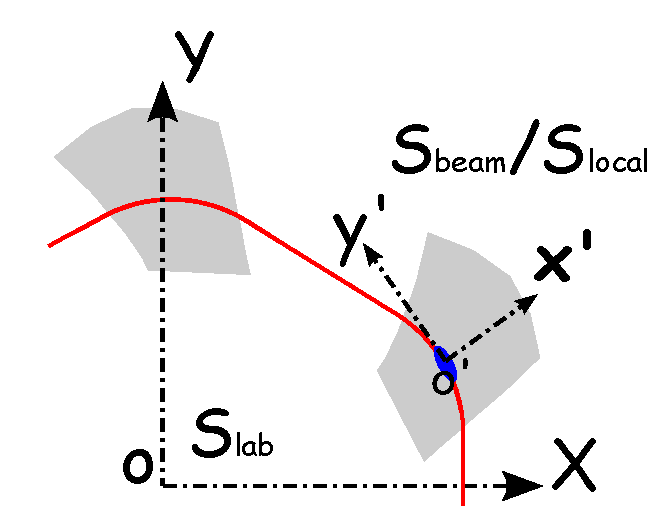
\includegraphics[width=8cm]{figures/SM-frame.pdf}}
    \caption{(Color) Schematic plot of the top view of the three coordinates frames. The red curve is the orbit of beam center, 
      the blue area represents beam shape, and the gray area is the hill region of magnetic field.}
    \label{fig:frame}
  \end{figure}

At each time step, in order to solve for the space charge fields, the frames $\bs{S}_{\RM{local}}$ and $\bs{S}_{\RM{beam}}$ are redefined according to current 6D 
phase space distribution, and all particles are transformed from $\bs{S}_{\RM{lab}}$ to $\bs{S}_{\RM{local}}$, 
then a Lorentz transformation is performed to transform all particles to $\bs{S}_{\RM{beam}}$.
The Poisson equation is then solved in frame $\bs{S}_{\RM{beam}}$. In a 3D Cartesian frame, the solution of the Poisson equation at point $(x,y,z)$ can be expressed by 
\begin{equation}\label{eq:Poten}
  \phi(x,y,z)= \frac{1}{4\pi\varepsilon_0}\int{G(x,x',y,y',z,z')\rho(x',y',z')dx'dy'dz'},
\end{equation}
with $G$ the 3D Green function 
\begin{equation}\label{eq:Green}
  G(x,x',y,y',z,z')= \frac{1}{\sqrt{(x-x')^2+(y-y')^2+(z-z')^2}}.
\end{equation}
assuming open boundary conditions.
The typical steps of calculating space charge fields using the Hockney's FFT algorithm \cite{Hockney:1} is sketched in Algorithm \ref{alg1:sc3d},
where the quantities with superscript $D$ (discrete) refer to grid quantities.

\begin{algorithm}
  \caption{3D Space Charge Calculation} 
  \label{alg1:sc3d}
  \begin{algorithmic}[1]
    \STATE \textbf{procedure} 3DSpaceCharge(In: $\rho$, $G$, Out: $\bs{E_{sc}}$,$\bs{B_{sc}}$)
       \STATE Create 3D rectangular grid which contains all particles, % and doubled it in each dimension, 
       \STATE Interpolate the charge $q$ of each macro-particle to nearby mesh points to obtain $\rho^D$, 
       \STATE Lorentz transformation to obtain $\rho^D$ in the beam rest frame $\bs{S}_{\RM{beam}}$,
       \STATE FFT $\rho^D$ and $G^D$ to obtain $\widehat{\rho}^D$ and $\widehat{G}^D$,
       \STATE Determine $\widehat{\phi}^D$ on the grid using $\widehat{\phi}^D = \widehat{\rho}^D \cdot \widehat{G}^D$,
       \STATE Use FFT$^{-1}$ of $\widehat{\phi }^D$ to obtain $\phi^D$,
       \STATE Compute $\bs{E}^D= -\nabla \phi^D$,
       \STATE Interpolate $\bs{E}$ at the particle positions $\bs{x}$ from $\bs{E}^D$,
       \STATE Perform Lorentz back transform to obtain $\bs{E_{\RM{sc}}}$ and $\bs{B_{\RM{sc}}}$ in  frame $\bs{S}_{\RM{local}}$ and transform back  to $\bs{S}_{\RM{lab}}$.
       \STATE \textbf{end procedure}
  \end{algorithmic}
\end{algorithm}
With respect to the external magnetic field two possible situations can be considered: 
in the first situation, the real field map is available on the median plane of the existing cyclotron machine using measurement equipment.
In view of the narrow gaps of magnets, in most cases concerning cyclotrons, the vertical field, $B_z$, is measured on the median plane ($z=0$) only.
Since the magnetic field outside the median plane is required to compute trajectories with $z \neq 0$, the field needs to be expanded in the $Z$ direction. 
According to the approach given by Gordon and Taivassalo \cite{Gordon:2}, by using a magnetic potential and measured $B_z$ on the median plane
at the point $(r,\theta, z)$ in cylindrical polar coordinates, the 3$rd$ order field can be written as    
\begin{eqnarray}\label{eq:Bfield}
  B_r(r,\theta, z) & = & z\frac{\partial B_z}{\partial r}-\frac{1}{6}z^3 C_r, \nonumber\\    
  B_\theta(r,\theta, z) & = & \frac{z}{r}\frac{\partial B_z}{\partial \theta}-\frac{1}{6}\frac{z^3}{r} C_{\theta}, \\     
  B_z(r,\theta, z) & = & B_z-\frac{1}{2}z^2 C_z,  \nonumber    
\end{eqnarray}
where $B_z\equiv B_z(r, \theta, 0)$ and  
\begin{eqnarray}\label{eq:Bcoeff}
  C_r & = & \frac{\partial^3B_z}{\partial r^3} + \frac{1}{r}\frac{\partial^2 B_z}{\partial r^2} - \frac{1}{r^2}\frac{\partial B_z}{\partial r} 
        + \frac{1}{r^2}\frac{\partial^3 B_z}{\partial r \partial \theta^2} - 2\frac{1}{r^3}\frac{\partial^2 B_z}{\partial \theta^2}, \nonumber  \\    
  C_{\theta} & = & \frac{1}{r}\frac{\partial^2 B_z}{\partial r \partial \theta} + \frac{\partial^3 B_z}{\partial r^2 \partial \theta}
        + \frac{1}{r^2}\frac{\partial^3 B_z}{\partial \theta^3},  \\
  C_z & = & \frac{1}{r}\frac{\partial B_z}{\partial r} + \frac{\partial^2 B_z}{\partial r^2} + \frac{1}{r^2}\frac{\partial^2 B_z}{\partial \theta^2}. \nonumber
\end{eqnarray}

All the partial differential coefficients are computed on the median plane data by interpolation, using Lagrange's 5-point formula.

In the other situation, 3D fields for the region of interest are calculated numerically by building a 3D model using commercial software 
during the design phase of a new cyclotron. In this case the calculated field will be more accurate, especially at large distances from the median plane i.e. a
full 3D field map can be calculated. For all calculations in this paper, we use the method by Gordon and Taivassalo \cite{Gordon:2}.

Finally both the external fields and space charge fields are used to track particles for one time step using a 4$th$ order Runge-Kutta (RK) integrator, in which 
the fields are evaluated for four times in each tracking step. Space charge fields are assumed to be constant during one tracking step,
because their variation is typically much slower than that of external fields. 
    
\section{NEIGHBORING BUNCH EFFECTS}
%1. self-consistent model using multi-bunch track strategy, advantage and disadvantage. 
%2. energy bin and rebin trick in cyclotron.
%3. new bunch injection trick. 
In cyclotrons the pattern of turn separation $\Delta R$ is affected by many factors. These include machine characteristics such as the magnetic field map, 
the voltage profile, the accelerating phase of the RF resonators  and initial centering conditions of the injected bunches. 
%The typical tendency is that  $\Delta R$ reduces gradually  with increasing beam energy.
Generally, in cyclotrons, $\Delta R$ reduces gradually  with increasing beam energy.
For machines like the PSI Injector\,II, $\Delta R$ stays sufficiently large from injection to extraction, and in such cases,  neighboring bunch effects are negligible. 
For others, like the PSI 590\,MeV Ring cyclotron under consideration in this section, $\Delta R$ decreases strongly during the course of acceleration resulting in the need to consider neighboring bunch effects in order to
obtain a precise description of the beam dynamics.

In our model, initially a single bunch with $N_p$ particles is injected and its average radial position $R_s$ is recorded. This bunch is tracked with space charge on. 
After exactly one revolution period $T_{r}$ the new radial position $R_e$ is recorded again. If the condition
\begin{equation}\label{eq:dR}
  \Delta R = R_e-R_s \le M \times r_{\RM{rms}},
\end{equation}
is fulfilled, (where $r_{\RM{rms}}=\sqrt{x_{\RM{rms}}^{2}+y_{\RM{rms}}^2}$ is beam rms size, $M$ is the parameter given by the user), 
the 6D phase space data $(x, p_x, y, p_y, z, p_z)$ at this time step is stored. 
After it is further tracked for another $T_{r}$, the code is switched to multi-bunch mode. 
A new bunch is injected by reading the 6D phase space data stored before and the two bunches are tracked simultaneously.
The third bunch is then injected in the same way after another turn, and so forth, until the maximum bunch number $N_B$ is achieved in the simulation. $N_B$ is also set by the user.
The underlying assumption for this is that all bunches have the same phase space distribution when they reach a certain position.
This is realistic and reasonable when the machine is running in a steady state.  
To the contrary, if the condition of Eq.\,(\ref{eq:dR}) is not fulfilled,
the code continues to track a single bunch until Eq.\,(\ref{eq:dR}) is valid.   
This fact is summarised in Algorithm~\ref{alg:mbi}.

\begin{algorithm}
  \caption{Multi-Bunch Injection Algorithm} 
  \label{alg:mbi}
  \begin{algorithmic}[1]
    \STATE \textbf{procedure} Injection(In: $N_B$, $M$) 
    \STATE Inject one bunch at radius $R_s$, total bunch number $j=1$,
    \STATE Track bunch  for One revolution period $T_{r}$,
    \STATE calculate radius $R_e$ and beam size $r_{\RM{rms}}$,
    \WHILE {($R_e-R_s > M \times r_{\RM{rms}}$)}
    \STATE     $  R_s = R_e$,
    \STATE     Track bunch for $T_{r}$, calculate $R_e$ and $r_{\RM{rms}}$,
    \ENDWHILE
    \WHILE {($j < N_B$)}
    \STATE Inject a new bunch, j++,
    \STATE Track all bunches for $T_{r}$,
    \ENDWHILE
    \STATE \textbf{end procedure}
  \end{algorithmic}
\end{algorithm}

Here another question arises. How many bunches should be simulated to evaluate neighboring bunch effects? 
  
\begin{figure}
    {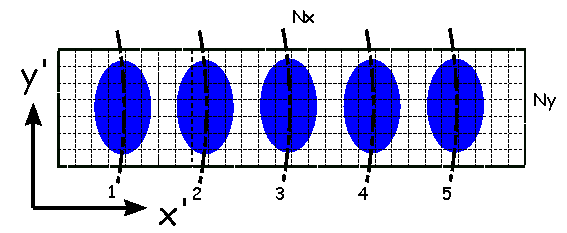
\includegraphics[width=8cm]{figures/SM-MultiBunch.pdf}}
    \caption{(Color) Schematic plot of the top view of 5 bunches and the grid of computation domain. The grid size on $X'-Y'$ plane is Nx$\times$Ny, and the broken lines represent the orbits of beam centers. }
    \label{fig:MultiBunch}
\end{figure}

In order to answer this question, let's first do a physical analysis for the case of 5 bunches, as shown schematically in Fig.\,\ref{fig:MultiBunch}.
The objective is to study the evolution of the center bunch, namely Bunch 3. 
Neighboring bunch effects are eventually derived from all the interactions of individual particles in the bunches. 
The electric field between two point charges is proportional to $1/r^2$, where $r$ is their distance. In this case, for Bunch 3, the sources
of neighboring bunch effects are mainly caused by the direct space charge force of Bunches 2 and 4 (of the first order), which are much stronger than 
those from Bunch 1 and 
5 (of the second order). However, Bunch 1 and 5 also have indirect impacts on Bunch 3, 
namely by their direct space charge force (of the first order) to the evolution of Bunch 2 and 4, respectively. 

In order to obtain a more accurate and consistent solution, one needs to employ more bunches. In theory, when the maximum bunch number $N_B$ equals the total turn number of the machine, one can eventually obtain the fully self-consistent solution of the problem within our model. 
In reality, it is not feasible  to simulate a full set of bunches, which typically range from 
several ten to several hundred.
The scale of particle number and the dimensions of the grid are beyond the capability of today's supercomputer resources.

A pragmatic approach is given by doing the simulation for 3 bunches and 5 bunches and comparing phase space results first. If the discrepancy in beam size is beyond 
the high limit of tolerance, one needs to do the simulation for 7 bunches, and compare its result with 5 bunches, and so forth. 
Eventually, with the proper setting of $N_B$ and $M$, neighboring bunch effects can be evaluated precisely.
For instance, the setting with $N_B=9, M=4.5$ gives convergent results for the PSI Ring cyclotron with 3\,mA beam current.
We will discuss this in more detail in the following section. 

In a multi-bunch simulation the energy of bunches in different turns is quite different. 
For a 9 proton beam simulation, if the kinetic energy of the first bunch $E_k=100~\text{MeV}$ and energy gain per turn $\Delta E_k=2~\text{MeV}$, 
the velocity difference of the first and last bunch is $6.5\%$.  
In this case there is no single rest frame in which the relative motions of 
particles are non-relativistic, as required by our scheme to calculate the space charge forces. Consequently it is not sufficient to use only one rest frame 
and a single Lorentz transformation. In order to calculate space charge fields more precisely, we introduce an adaptive binning technique.
First we create the same amount of energy bins as the bunches, and alculate the average relativistic factor $\bar{\gamma_i}$ for the i$th$ bunch with $N_p^i$ simulation particles
\begin{equation}\label{eq:dR1}
  \bar{\gamma}_i = \frac{\sum_{j=1}^{N_p^i}\sqrt{1+p_{j,x}^2+p_{j,y}^2+p_{j,z}^2}}{N_p^i}.
\end{equation}
Then every particle is grouped into the energy bin whose $\bar{\gamma_i}$ is closest to its $\gamma$. In this way, the energy spread of each bin is small and the relative motions of the particles in the same bin are non-relativistic.
After binning we perform the Lorentz transformation, calculate the space charge field and perform back-transformation for each bin respectively. 
Finally the field data is summed up to give  the total space charge force imposed on each particle.

The energy spread of the bunches can be large (MeV range), especially in cyclotrons without flat-top cavities, and at large radii. This may result in an overlap of 
energy distributions of neighbouring bunches, and hence the energy bins have to be recalculated i.e.\ all particles need to be regrouped after each evolution.
It is worth noting that, in cyclotrons, the energy difference of neighboring bunches changes  with the increasing radius.
Therefore the energy difference of the neighboring bins is not constant. Specifically the energy difference between the i$th$ and i-1$th$ bins, $\Delta\bar{E}_{i,i-1}$, 
differs with the energy difference between the i+1$th$ and the i$th$ bins $\Delta\bar{E}_{i+1,i}$.

\section{IMPLEMENTATION WITHIN THE \opal \  FRAMEWORK}
%1. Brief introduction of OPAL characteristic.
%2. The Hierarchical layout of code.%

%3. Introduction of functionality of OPAL-cycl.

The above model and algorithm are implemented in the object-oriented parallel PIC code \opalcycl. 
\opalcycl \  is one of the flavors of the \opal \ (Object Oriented Parallel Accelerator Library) framework \cite{opal:1}. 
This framework is a powerful tool for charged-particle optics in general accelerator structures and beam lines using the MAD languages with extensions.
\opal ~ is  based on the CLASSIC \cite{Classic:1} library and the IP$^2$L framework \cite{ippl:1}. The CLASSIC library is a C++ class library which provides services for building portable accelerator models and algorithms and input 
language to specify complicated accelerator systems in general. IP$^2$L is an Object-Oriented C++ class library which provides abstractions for particles and structured field calculation
in a data-parallel programming style. It provides an integrated, layered system of objects. The upper layers
contain global data objects of physical/mathematical quantities, such as particles, fields and matrices of meshes and typical methods
performed on these objects such as differential operators and multi dimensional FFT's. The lower layers contain the object's relevant to parallelization such as data distribution, domain decomposition, communication among processors, load balancing and chained-expression optimization. Statistical data, such as root mean square (rms) quantities, are computed on the fly (in situ) and stored in conjunction with phase space and
field data in the H5Part \cite{H5part:1} file-format. In a post processing step the data  can be analyzed
using the visualization tool H5PartRoot \cite{h5partroot:1}.
%(\url{http://amas.web.psi.ch/tools/H5PartROOT/index.html}).

In addition, apart from the multi-particle simulation mode, \opalcycl \  also has two other serial tracking modes for conventional cyclotron machine design. 
One mode is the single particle tracking mode, which is a useful tool for 
the preliminary design of a new cyclotron. It allows to compute  basic parameters, such as reference orbit, phase shift history,
stable region and matching phase ellipse. The other one is the tune calculation mode, which can be used to compute the betatron oscillation frequency 
$\nu_r$ and $\nu_z$. This is useful for evaluating 
the focusing characteristics of a given magnetic field map. 

A more detailed description of the hierarchical layout, the parallelization and the implementation issues of the \opal \  framework and \opalcycl \  code
can be found in the User's Reference Guide \cite{opal:1}.  


\section{PERFORMANCE TEST AND VALIDATION}
In order to evaluate the performance and to benchmark the functionalities of the newly developed code, we performed different types of simulations on
 the 72\,MeV Injector\,II cyclotron of PSI, which has been studied intensively before. Some results are presented in this section. 

\subsection{Single particle tracking and tune calculation}
In theory, there is an eigen-ellipse for any given energy in a cyclotron under stable conditions. Only when the initial phase space
matches this eigen-ellipse, the oscillation of the beam envelope amplitude will be minimal and the transmission efficiency will be maximal.
In the present test, the eigen-ellipse at 2\,MeV kinetic energy was calculated using the single particle tracking mode of \opalcycl.  
The result is compared to FIXPO \cite{FIXPO:1,joho:2}, the orbit integration program used at PSI to design the Injector II and the Ring cyclotron.
In Fig.\,\ref{fig:Eigen} the matched radial ellipse with an initial offset of $x=2.0{\RM{\,mm}}$, $p_x=0.0{\RM{\,mrad}}$ at the symmetry line of the sector field is shown.
Good agreement is obtained when the time step is set to 1\,ps in \opalcycl, although FIXPO uses a different tracking algorithm with the azimuthal angle as
the independent variable.
\begin{figure}
  {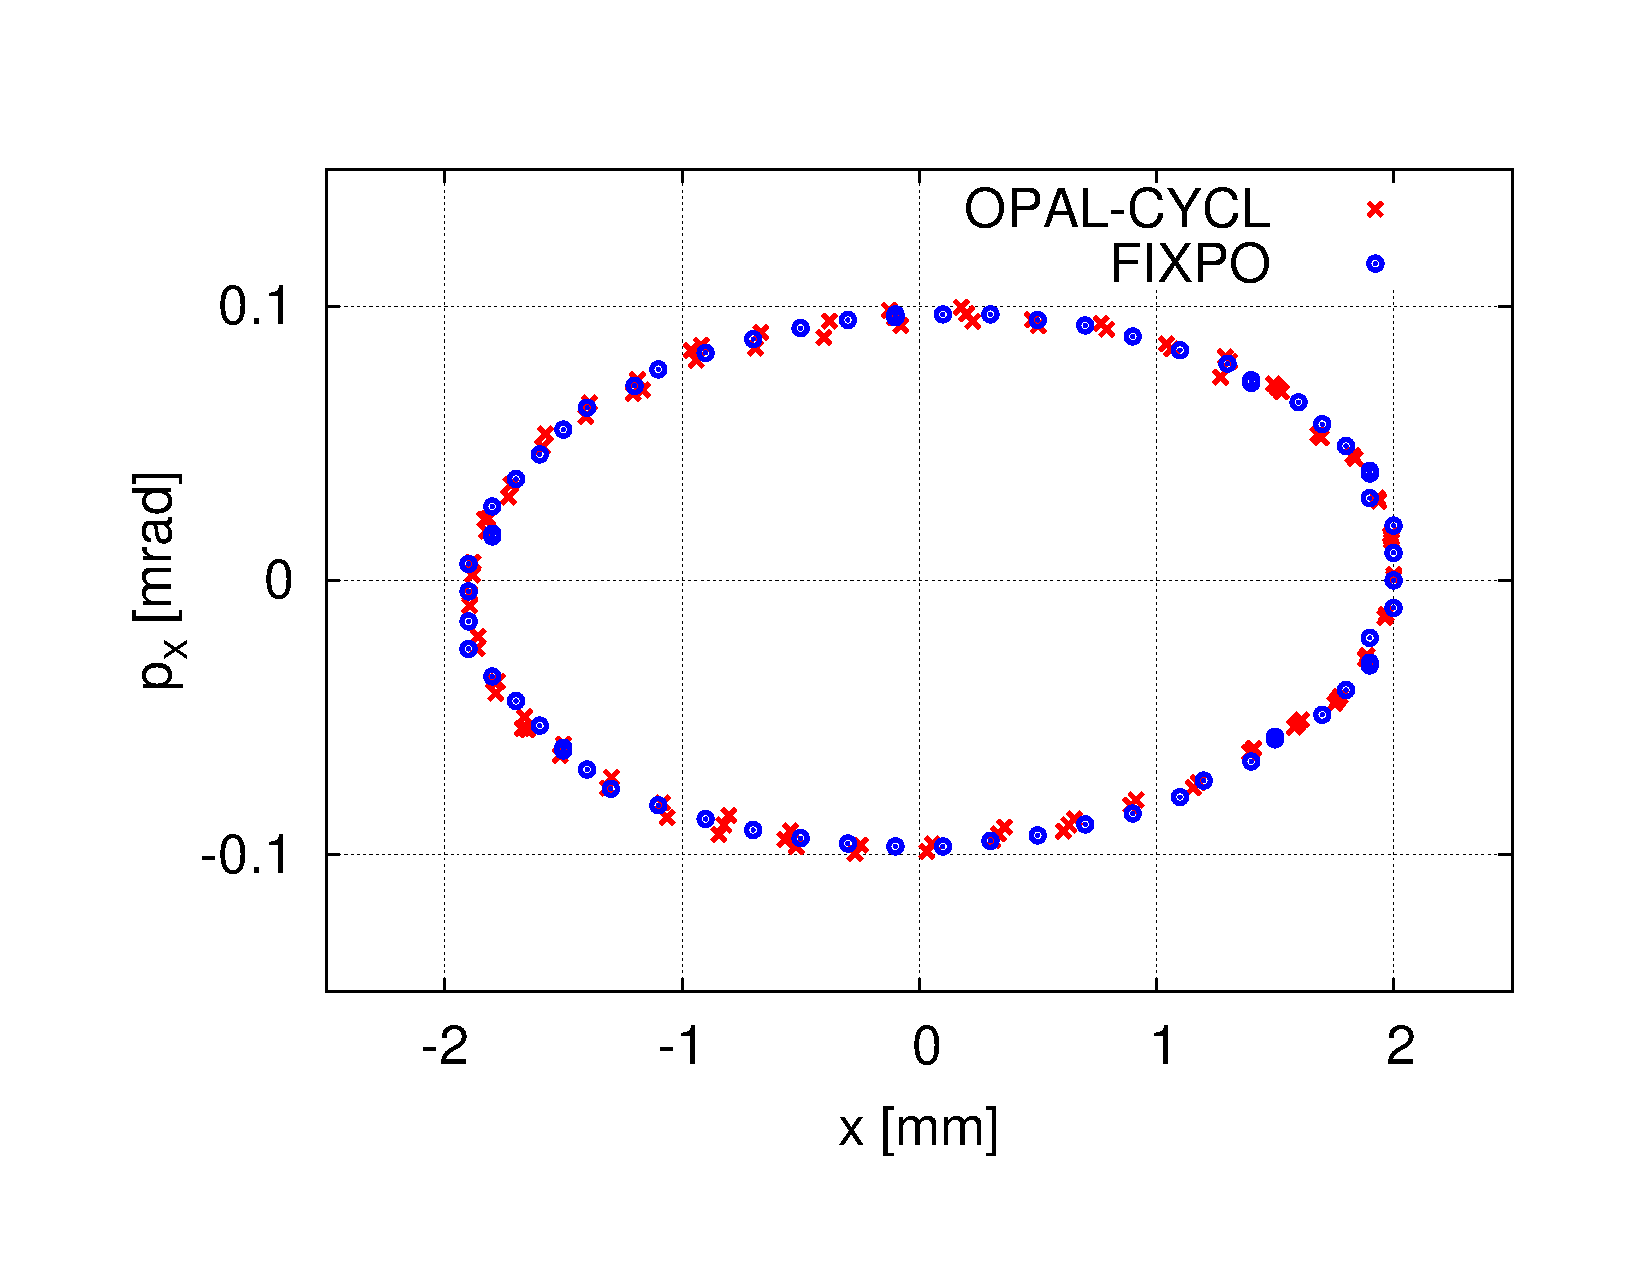
\includegraphics[width=8cm,trim=2.5cm 2.5cm 2.5cm 2.5cm]{figures/RadialEigen_Inj2.pdf}}
  \caption{(Color) Radial eigen-ellipse of 2\,MeV at the symmetric line of a magnet in Injector\,II cyclotron.}
  \label{fig:Eigen}
\end{figure}

The tune diagram of Injector\,II was computed using the tune calculation mode of \opalcycl, as shown in Fig.\,\ref{fig:nurnuz_Inj2}.
The result from FIXPO and \opalcycl \ are again in good agreement even though different numerical algorithms are used.% to calculate the tunes. 
\begin{figure}
  {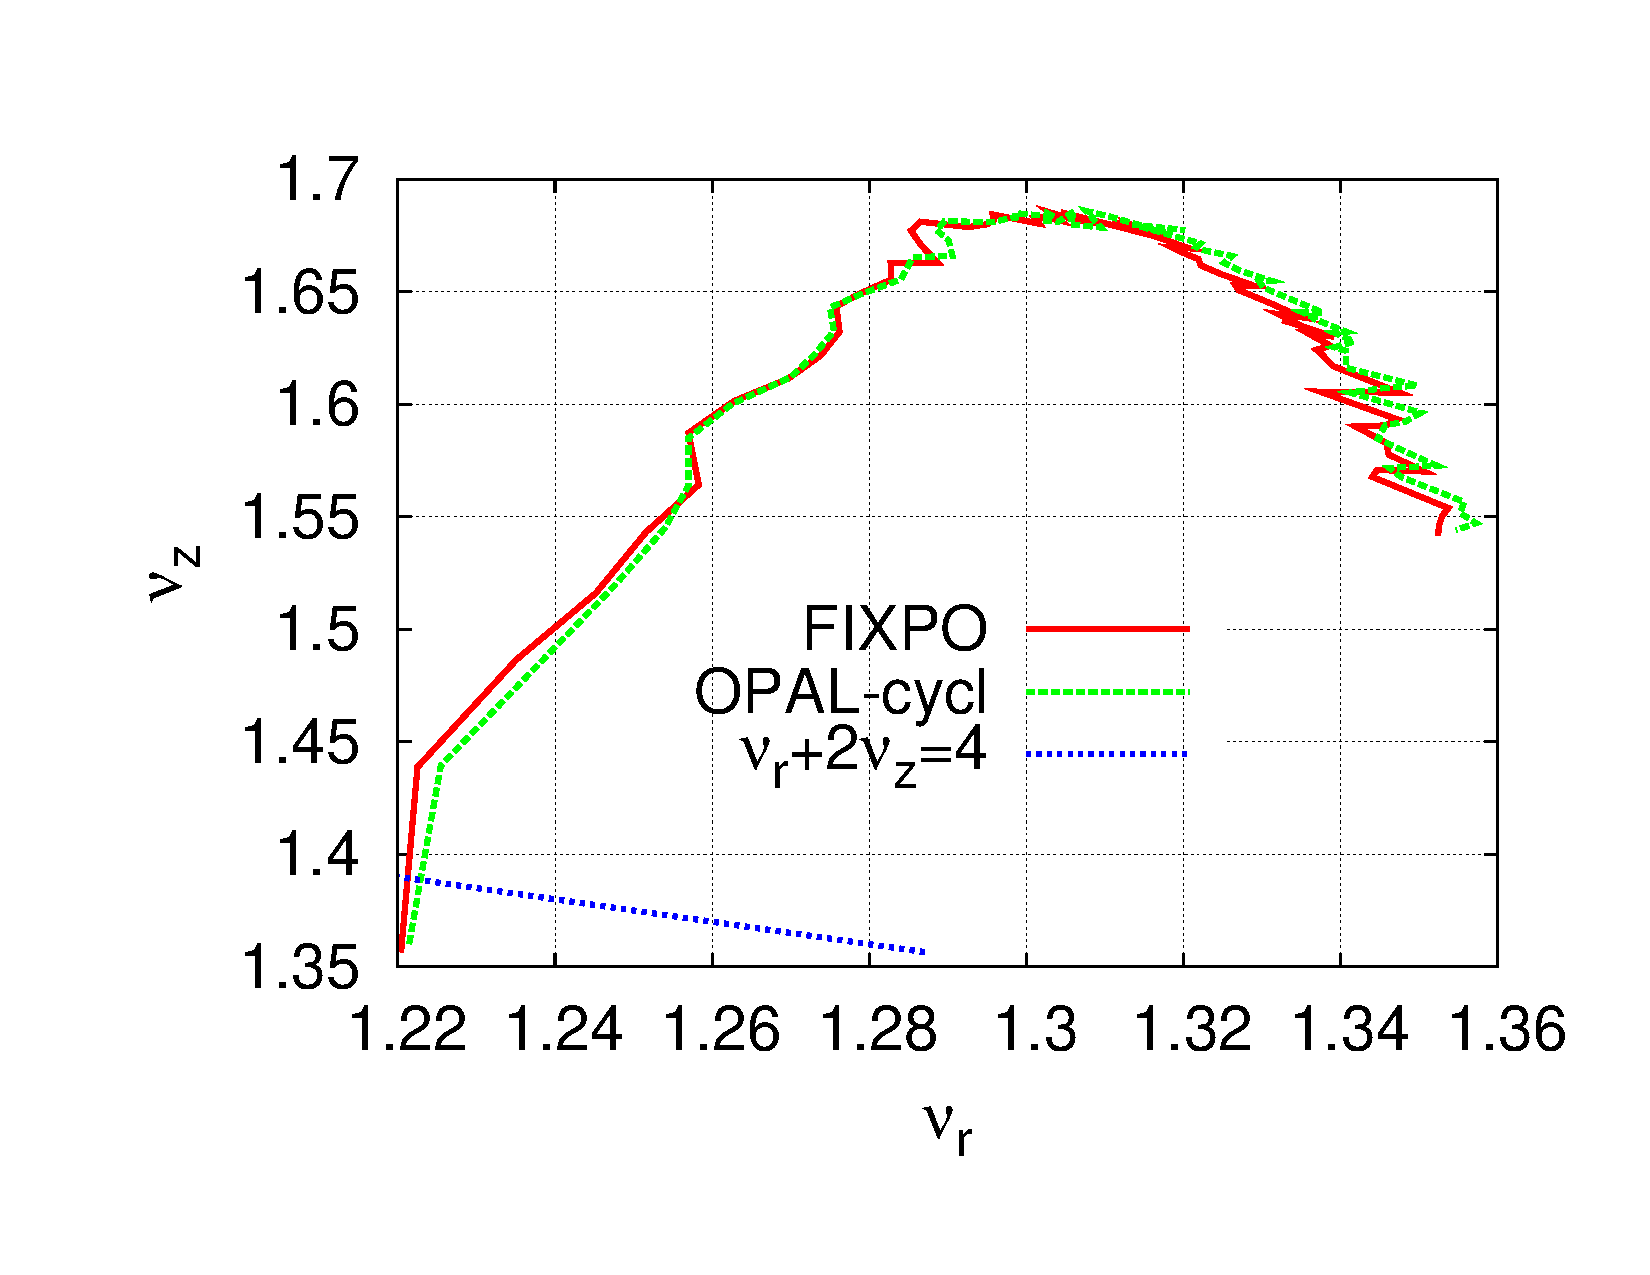
\includegraphics[width=8cm,trim=2.5cm 2.5cm 2.5cm 2.5cm]{figures/nurnuz_Inj2.pdf}}
  \caption{(Color) Tune diagram of Injector\,II cyclotron, compared with FIXPO code.}
  \label{fig:nurnuz_Inj2}
\end{figure}

The field interpolation scheme, particle tracking and tuning calculation functionalities are validated substantially by the above tests. 
\subsection{Parallel scalability test}
In order to observe the parallel scalability of the code, we have performed a detailed comparison of time consumption using a different number of processors. 
In this test, 1\,million particles are used to track 200 time steps on the Injector\,II. The initial beam has a Gaussian
type distribution. The grid size is $64 \times 64 \times 64$ which is decomposed onto a two dimensional grid of processors. All the intermediate phase space data is dumped into 
a single H5Part file. The dynamic load balancing frequency as well as the phase space dumping frequency are set to 10.
The results are shown in Fig.\,\ref{scalability}.
\begin{figure}
  {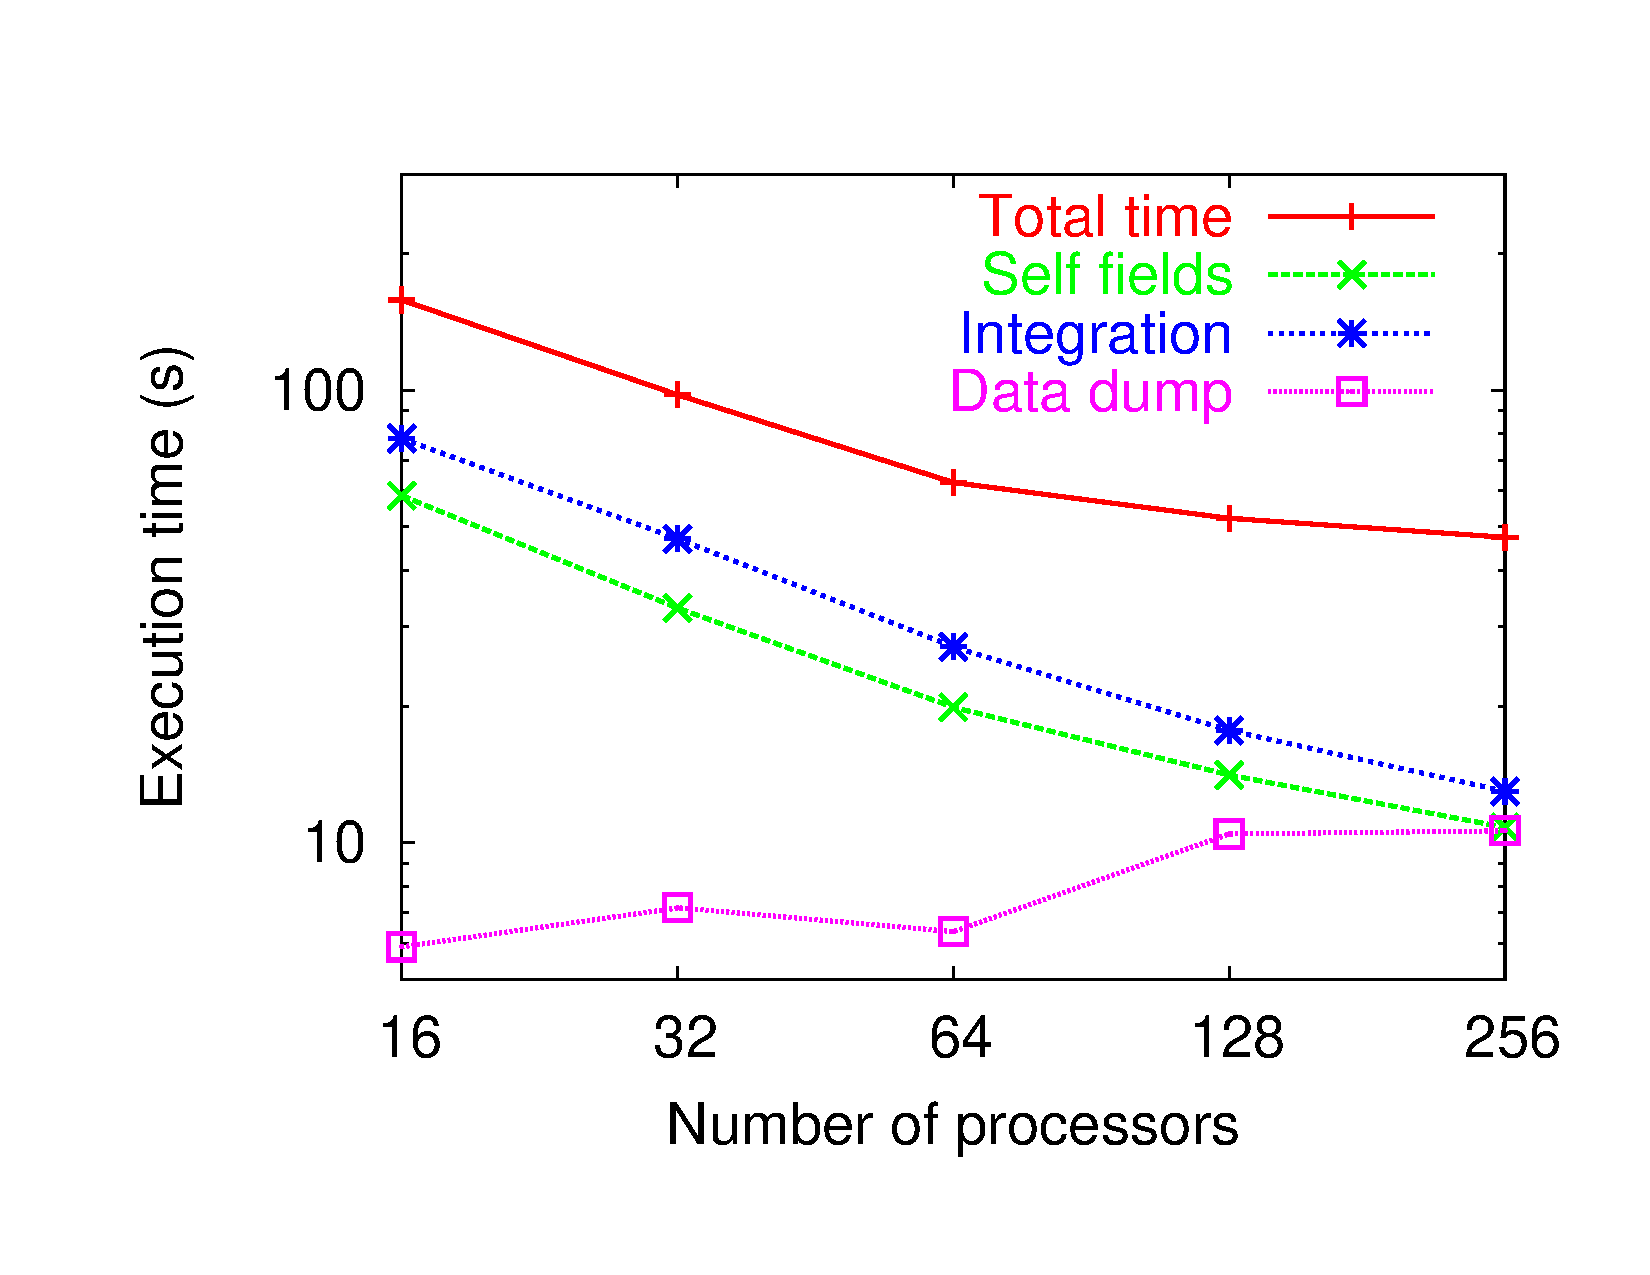
\includegraphics[width=8cm,trim=0cm 0cm 0cm 0cm]{figures/Timing64mesh.pdf}}
  \caption{(Color) The time consumption as a function of processors on Cray XT3, CSCS.}
  \label{scalability}
\end{figure}

We can see that good scalability is achieved up to 128 processors. When the number of processors reaches 128, the time consumption of the phase space dumping starts to become significant for the total computation time.
The reason is that the data is dumped into a single file and the data exchange between root node and other nodes increases significantly.
Nevertheless, the scalability of the space charge solver and the particles integrator still benefit from a large number of processors.

\subsection{Stationary Round Distribution in the PSI Injector\,II}
Space charge effects usually result in an increase in beam size and emittance. That is detrimental to beam dynamics. 
However there are cases, where space charge effects can actually play a positive role. The PSI Injector\,II cyclotron is a space charge dominated machine, in which a very compact 
stable beam is developed within the first several turns. Thereafter, the charge distribution stays at an extremely narrow phase width (about $2^\circ$), this stationary situation
remains essentially unchanged until extraction. This is due to the combined effect of the strong coupling between the
radial and longitudinal directions in the cyclotron and the space charge when the beam current increases above 1\,mA. S. Adam first reproduced this phenomenon by 
using the serial two-dimensional code PICN \cite{Adam:1}. PICN is based on the Needle model, which treats the beam as 
an ensemble of changed vertical needles with the same height as the beam. In this model, the vertical motion of particles is separated from the horizontal 
component and the internal motion within needles is neglected. In order to validate the space charge solver module of our code, we performed the 1\,mA, 3\,MeV coasting beam simulation on this machine and compared the result with PICN.  

We used the same initial distribution as in Ref. \onlinecite{Adam:3}.
$2\sigma_{\RM{longitudinal}} = 13.4 {\RM{\,mm}}$ ( $15^\circ$ phase width), $2\sigma_{\RM{transverse}} = 2.52 {\RM{\,mm}}$. 
The initial emittances of the radial and azimuthal directions are set to zero. 
In the vertical direction, $2\sigma_z = 4{\RM{\,mm}}$, $2\sigma_{p_z} = 3.68{\RM{\,mrad}}$. 
The total macro-particles number is 1\,million.  Fig.\,\ref{fig:coasting1mAA} shows the top view of beam shape in the local beam frame.
We can see that a stable core is developed after about 10 turns, which is faster than the formation of stable haloes.

When comparing Fig.\,\ref{fig:coasting1mAA} with Fig.\,3 and Fig.\,4 in Ref. \onlinecite{Adam:3} calculated by PICN, we can find the results agree with each 
other qualitative. Both of these two codes predict the formation of a compact stable core and  wide haloes after 40 turns.
However, there exist visible differences. PICN gives out a perfect ``round'' charge density distribution of core and \opalcycl\ gives out a not so perfect round one, namely, the longitudinal size of the core is about 2\,mm longer than the transverse size. The difference should mainly come from the different physics models used in the two codes.
In PICN all particles in close proximity to the horizontal plane are represented by a single ``needle''; in \opalcycl\  only those particles close to one other in configuration space are represented by a single macro-particle. The
latter is believed to be more realistic and accurate. 

We conclude from this comparison that \opalcycl\ can reliably reproduce the stable ``round'' beam formation caused by space-charge effects in Injector\,II and hence can accurately  reproduce the single bunch dynamics in cyclotrons.

\begin{figure*}
    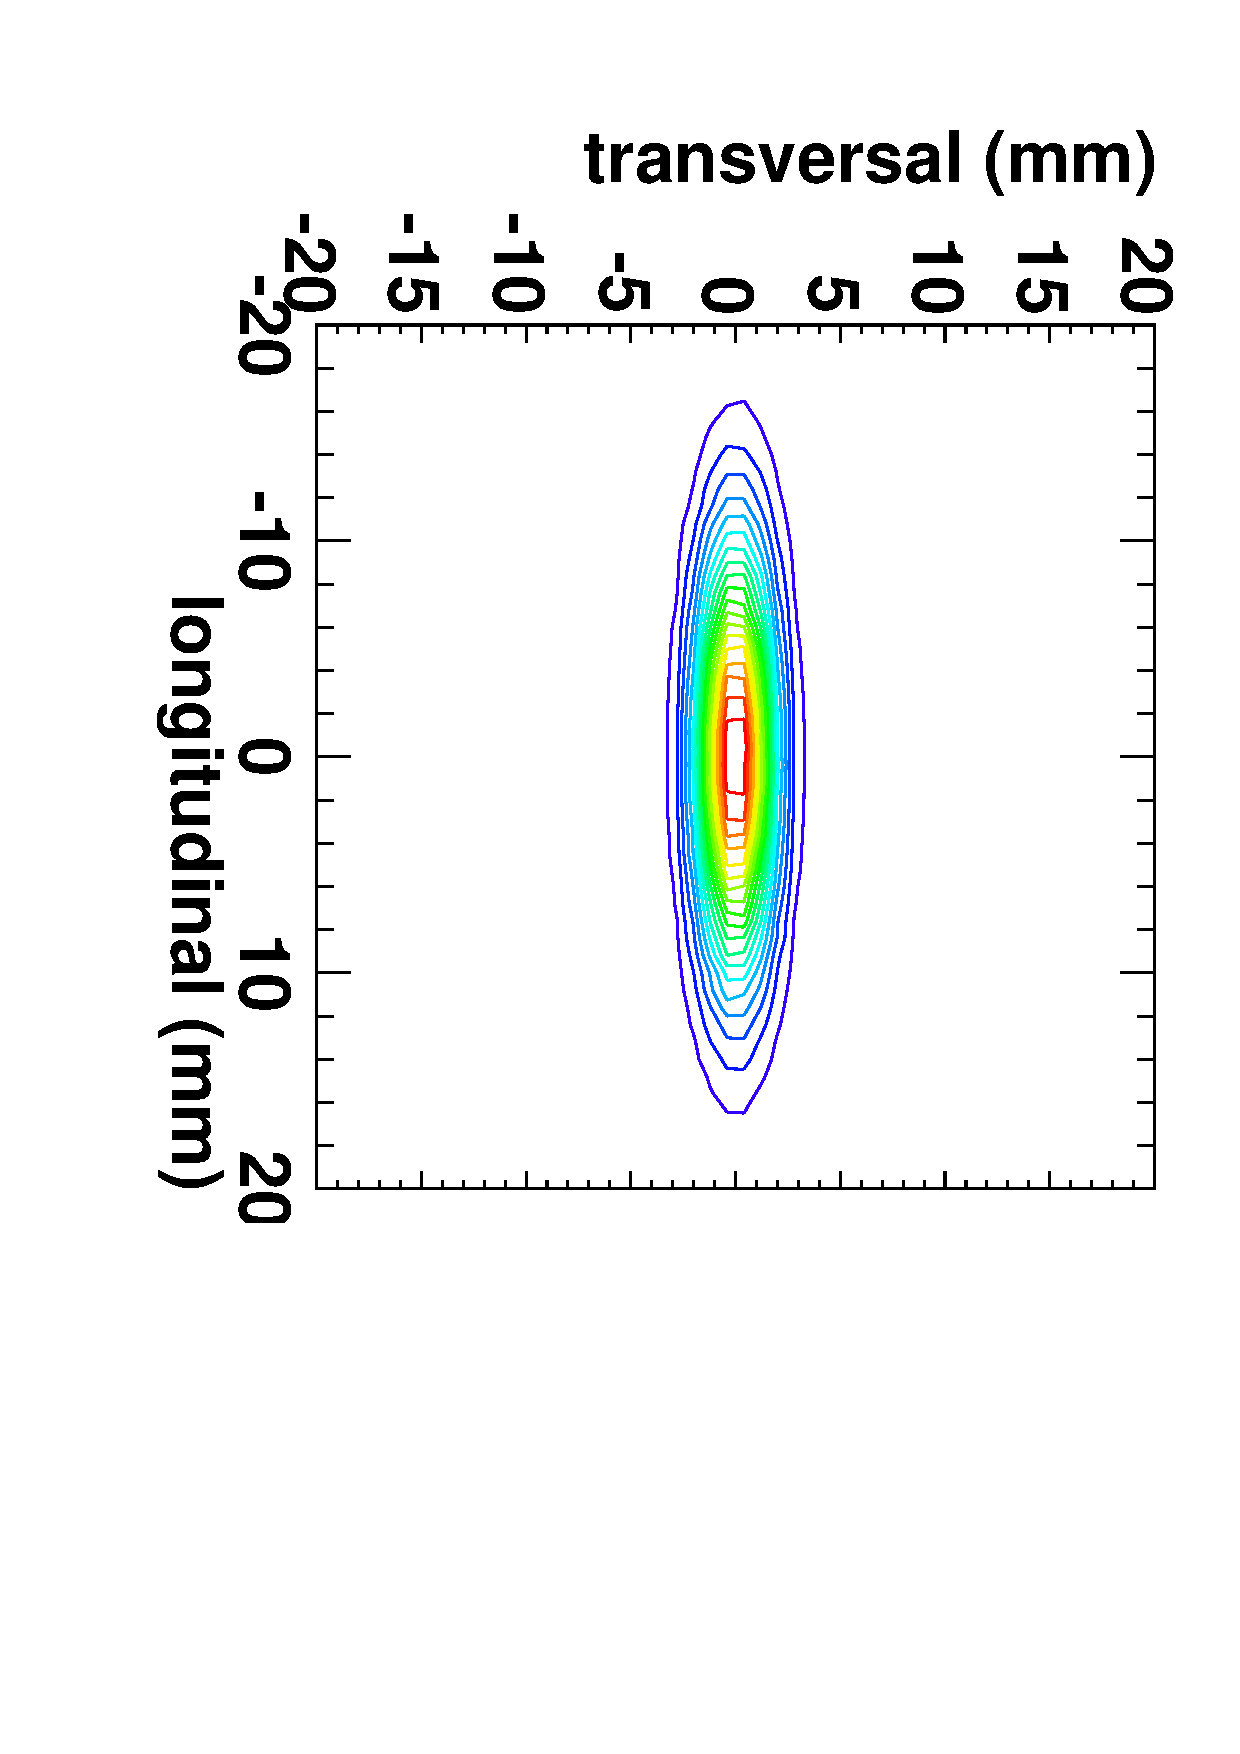
\includegraphics[angle=90,width=0.3\linewidth]{figures/Inj2/1mA0.pdf}
    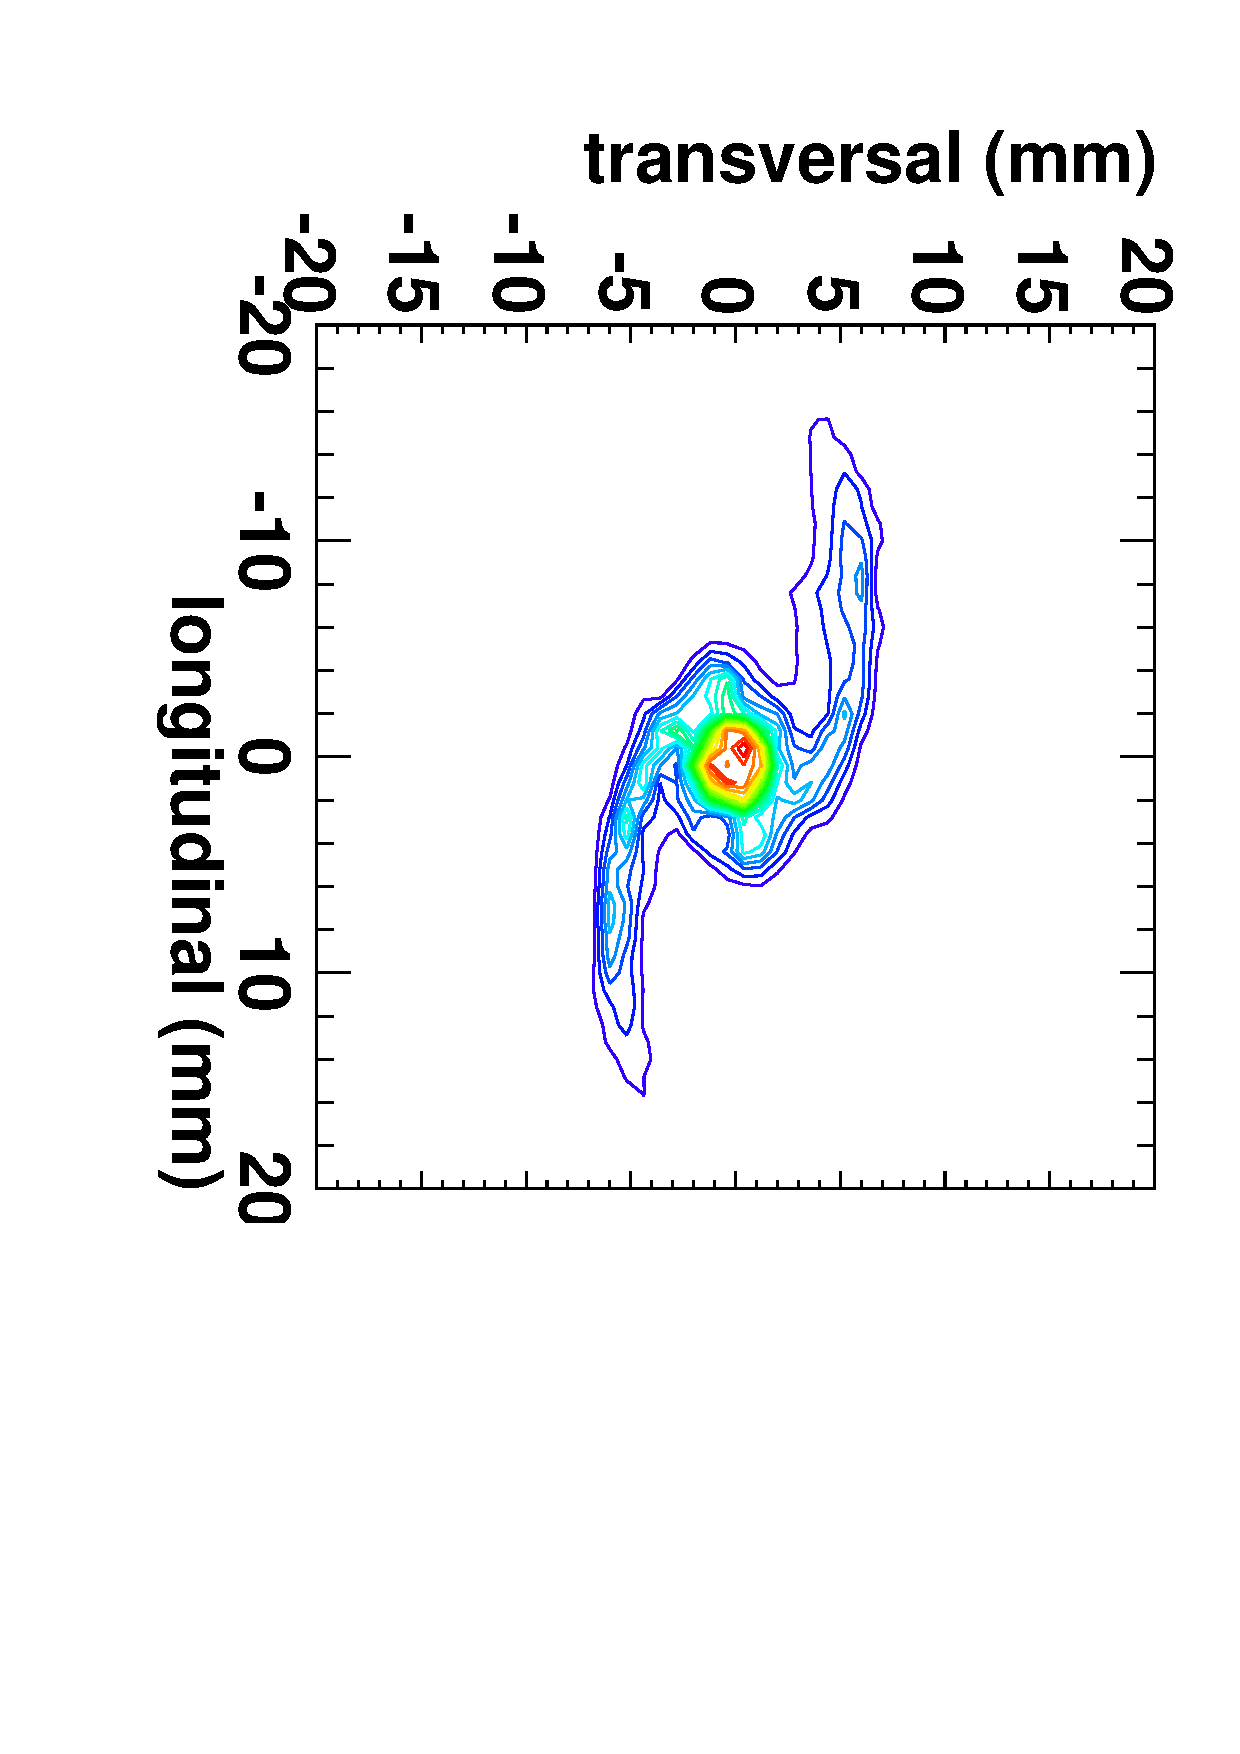
\includegraphics[angle=90,width=0.3\linewidth]{figures/Inj2/1mA5.pdf}
    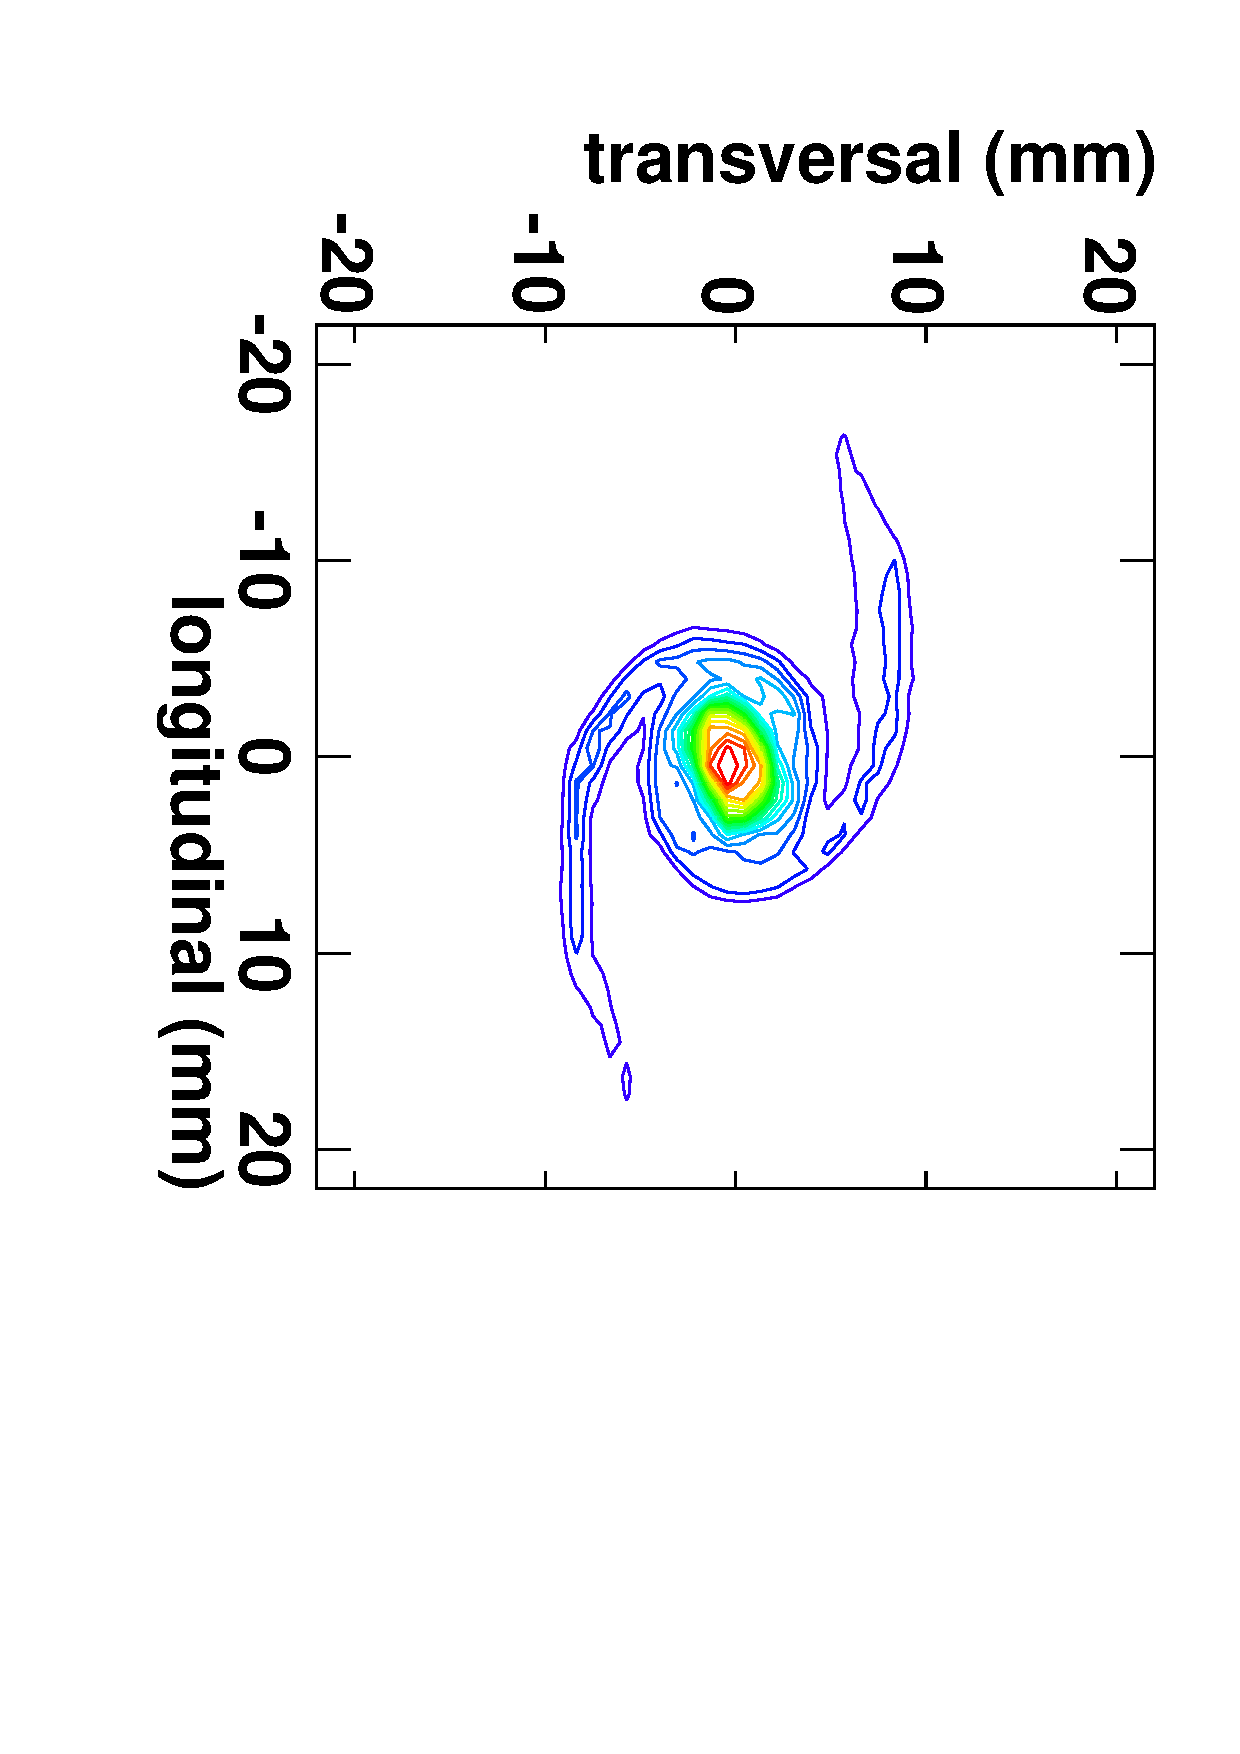
\includegraphics[angle=90,width=0.3\linewidth]{figures/Inj2/1mA10.pdf}
    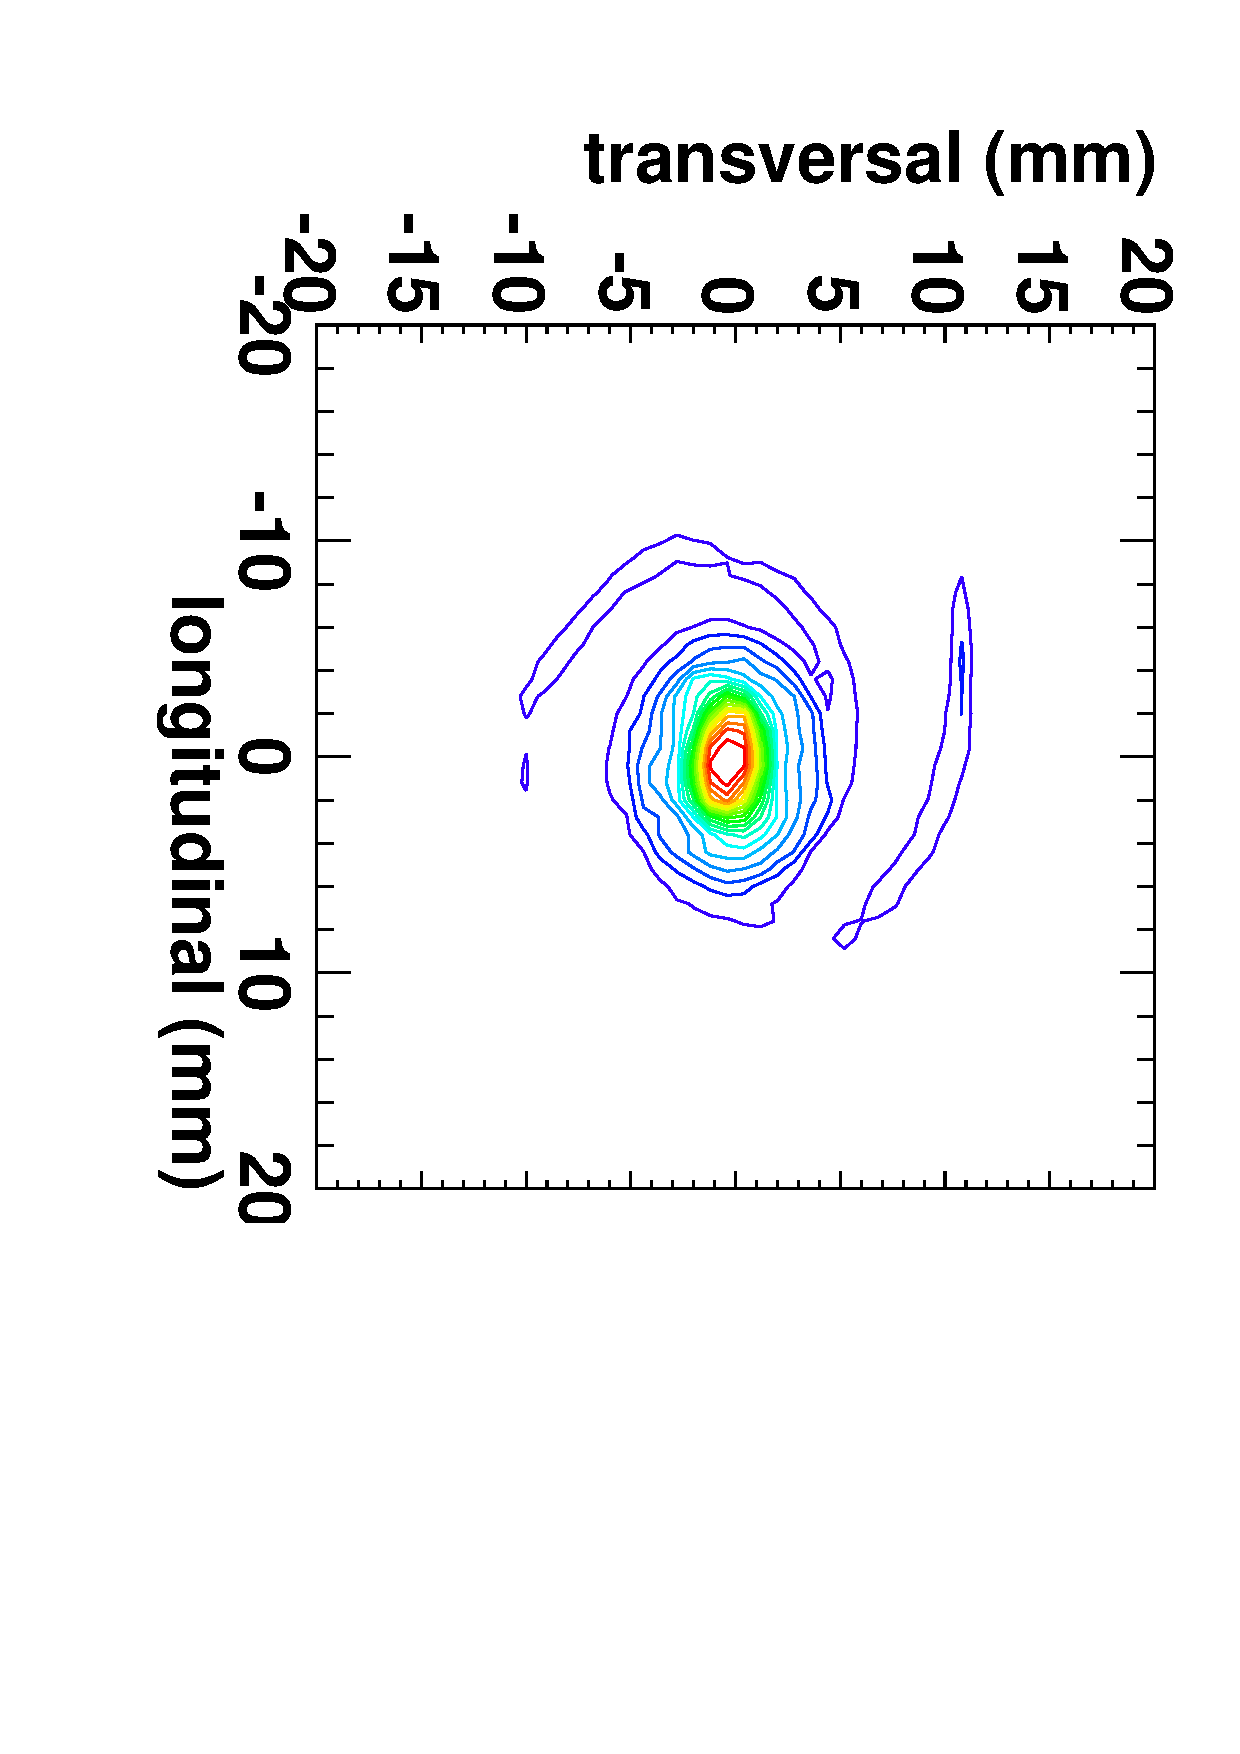
\includegraphics[angle=90,width=0.3\linewidth]{figures/Inj2/1mA20.pdf}
    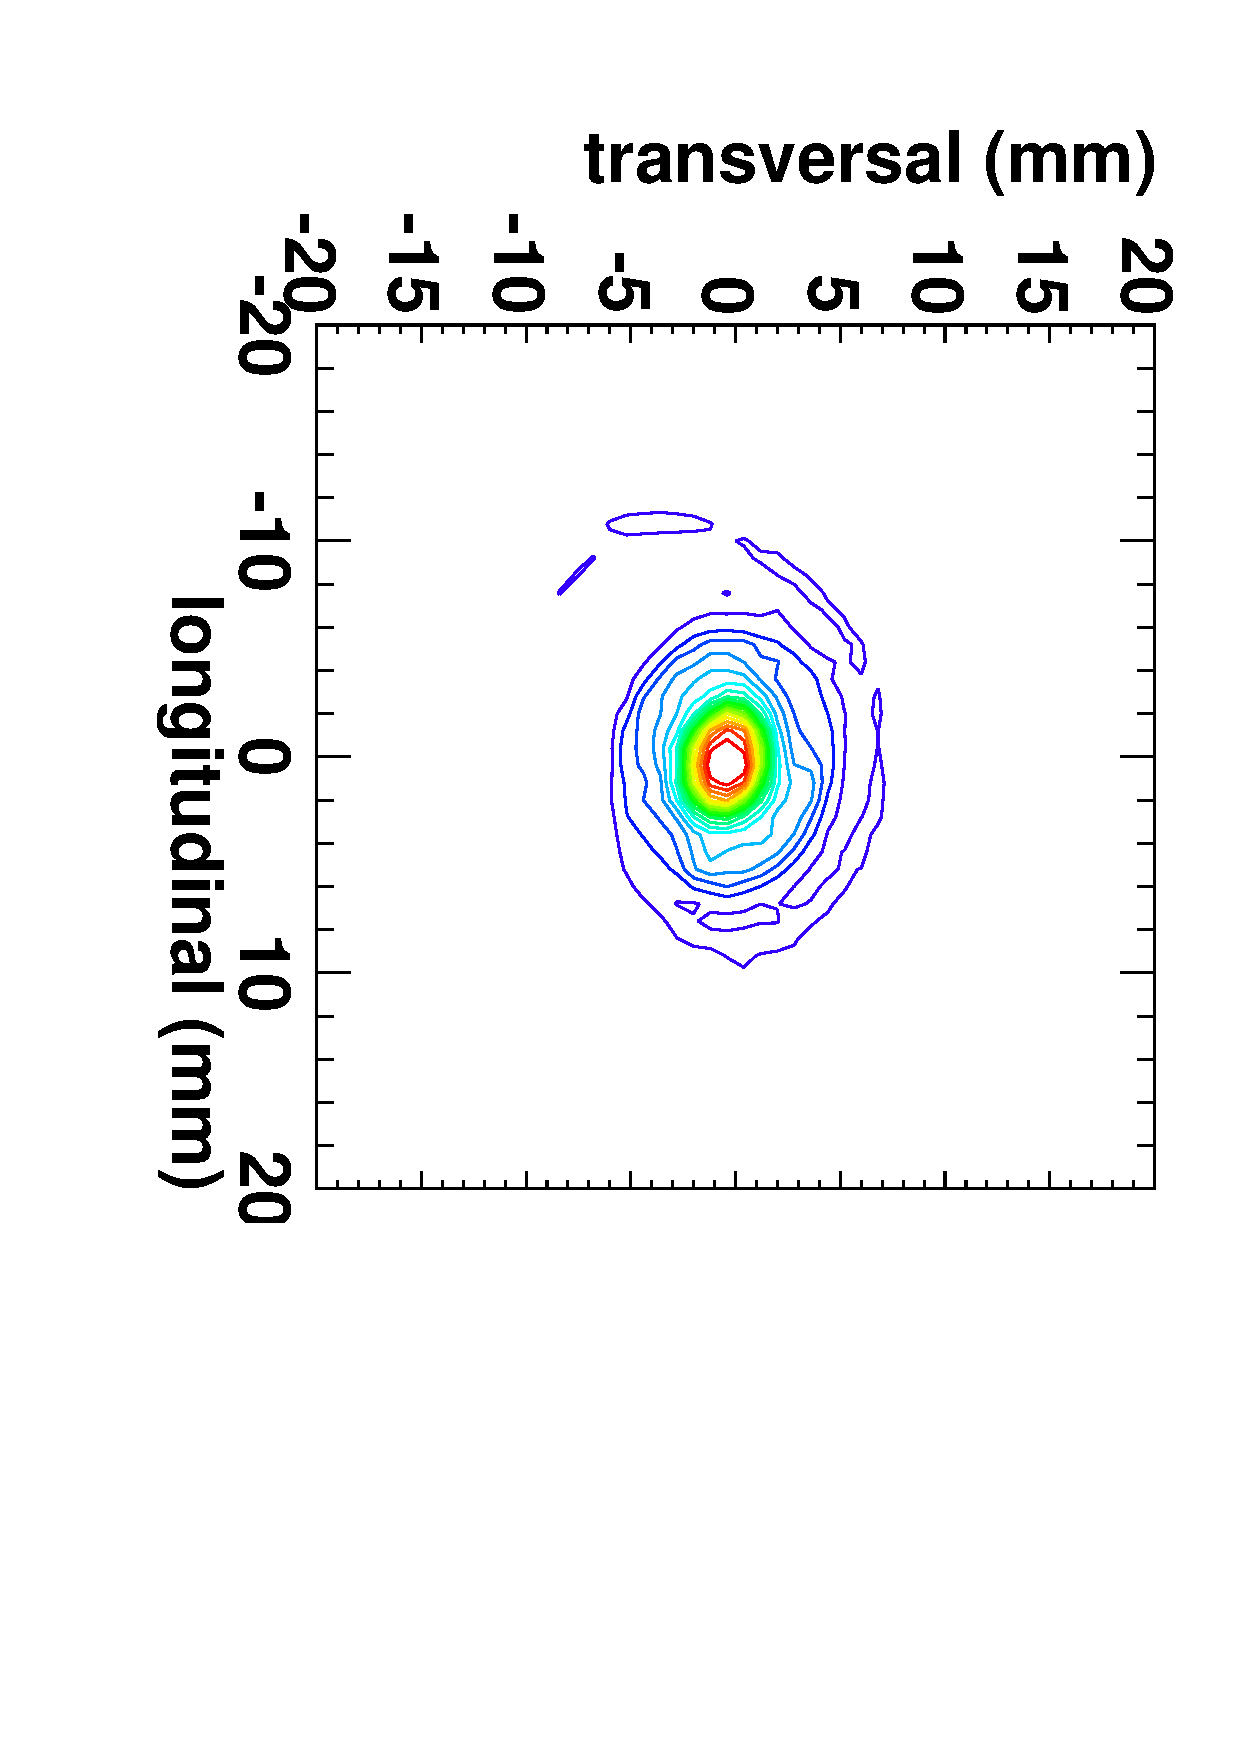
\includegraphics[angle=90,width=0.3\linewidth]{figures/Inj2/1mA30.pdf}
    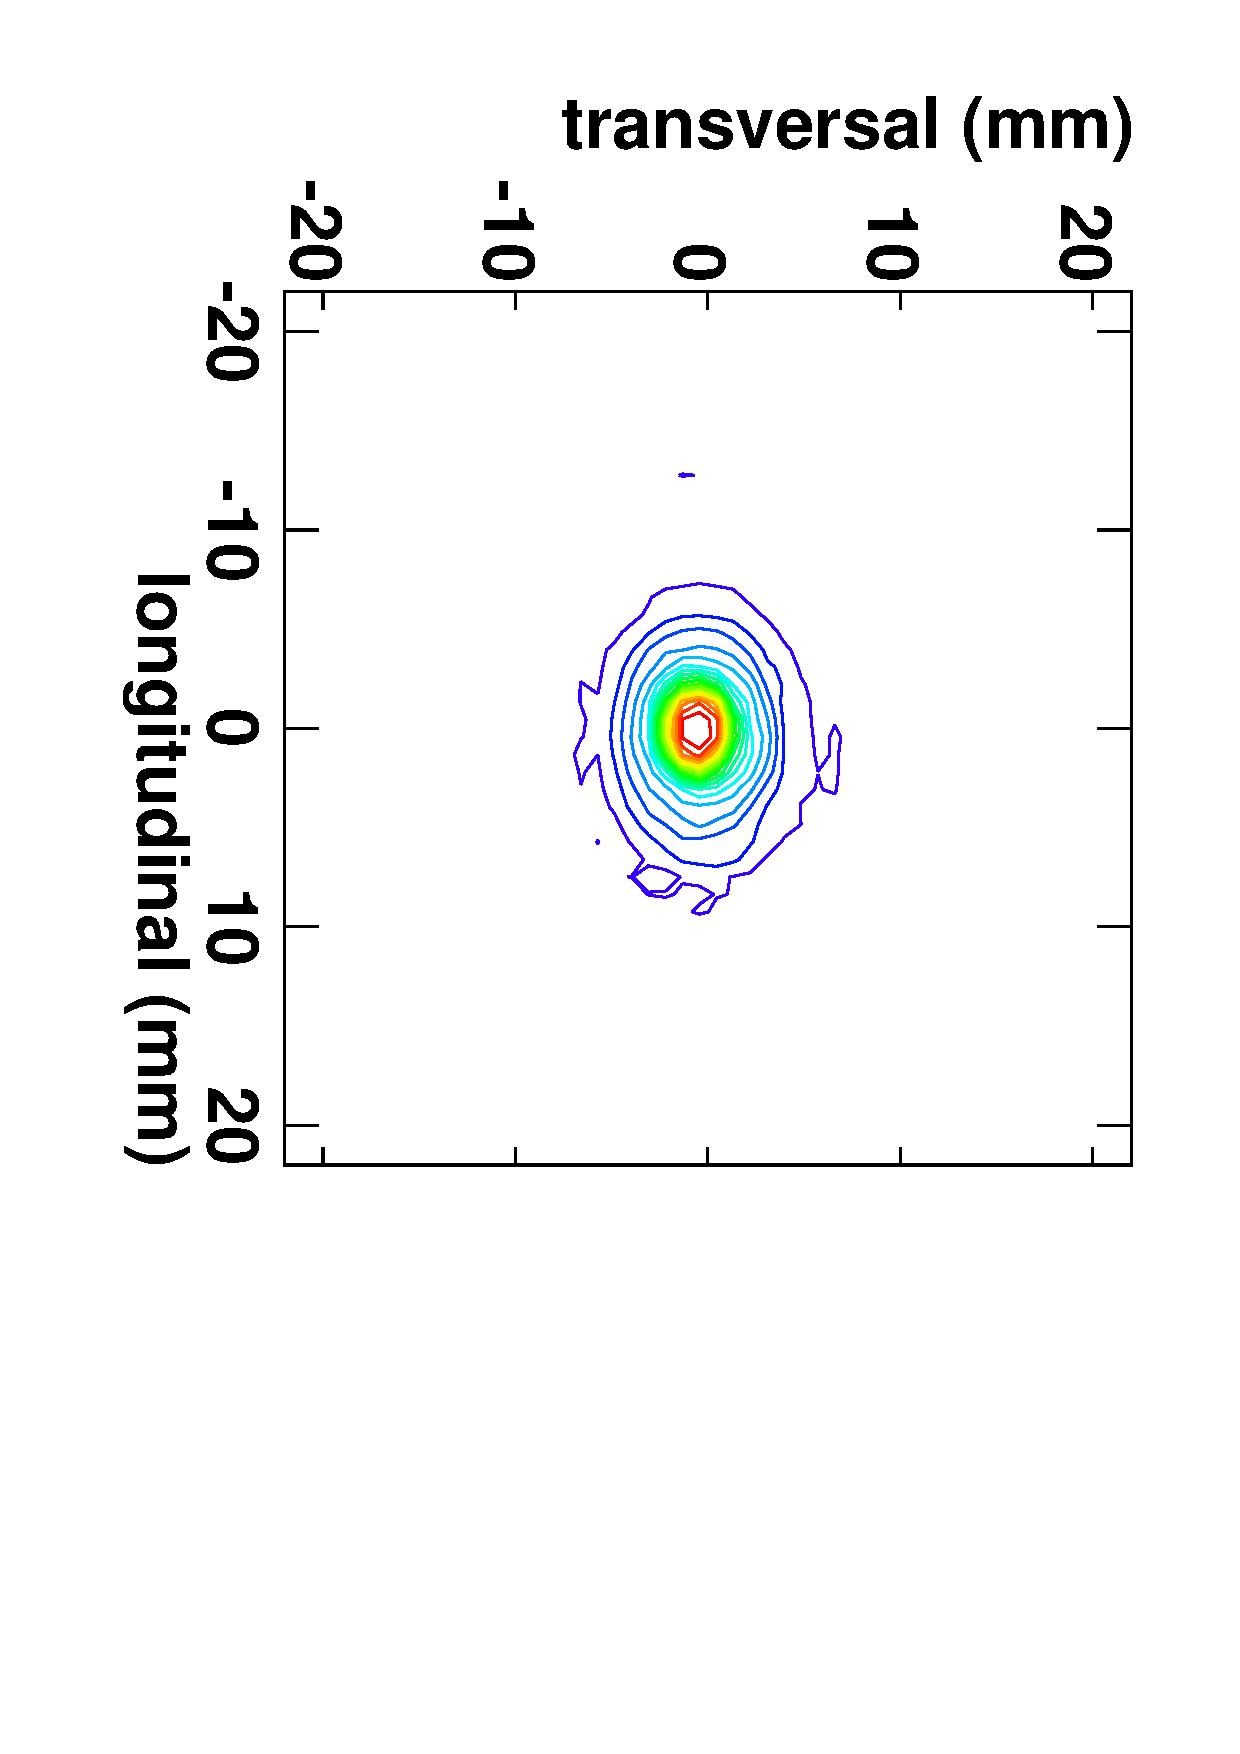
\includegraphics[angle=90,width=0.3\linewidth]{figures/Inj2/1mA40.pdf}
    \caption{(Color) Top view of a 1\,mA, 3\,MeV coasting beam in PSI Injector\,II in the local frame ${\bs{S}_{\RM{local}}}$ of PSI Injector\,II. 
      Up: turn 0, 5, 10. Down: turn 20, 30, 40. To compare with figures in Ref. \onlinecite{Adam:3}, 
      the beam's transport direction is along the negative direction of the abscissa axis.}
    \label{fig:coasting1mAA}
\end{figure*}


%\subsection{Transverse tune spread in Injector\,II}

%A number of references give the theoretical formula of the tune shift of linear-space-charge-equivalent beam or K-V equivalent beam in synchrotron theory\cite{Laslett:1,Baartman:2}.
%When the nonlinear space charge is taken into account, the values of tune shift of individual particles are different and on the transverse tune diagram the transverse tune 
%is not a single point but rather an area. Because of the complexity, it is impossible to obtain this area using theoretical formula.

%As the second example of multi-particle simulation in Injector\,II, \opalcycl \ was used to calculate the incoherent tune of 5, 10, 35 and 60 MeV for different beam current. 
%In the simulation, a coasting Gaussian beam of one million macro-particles with was tracked for 130 turns. 
%Afterward, 2000 samples particles at different position in phase space were chosen to evaluate the tune spread. 
%Because for all beam current levels, the beam get its stable state after 30 turns,
%the data from the 30th turn to 130th turn were used to do Lomb-Scargle periodogram analysis and the frequencies of individual particles were obtained.
%The resulting tune diagram are shown in Fig.\,\ref{fig:tuneSC}. 

%According to the result, tune spread is still small comparing with the bare tune of external field, 
%which means in this separated sector cyclotron the external focusing force are much stronger than space charge force 
%at beam current level of milliampere in both vertical and radial direction. 
%Therefore from the view of facusing, there is enough space for Injector\, II to increase its beam current to higher level. 
%We also can see that the area of tune spread is shrinked gradually along with the the increase of the energy because the space charge force become smaller at higher energy.  

%\begin{figure*}
%    \includegraphics[width=0.49\linewidth,trim=2.5cm 2.5cm 6cm 0cm]{figures/nurnuz-5MeV.pdf}
%    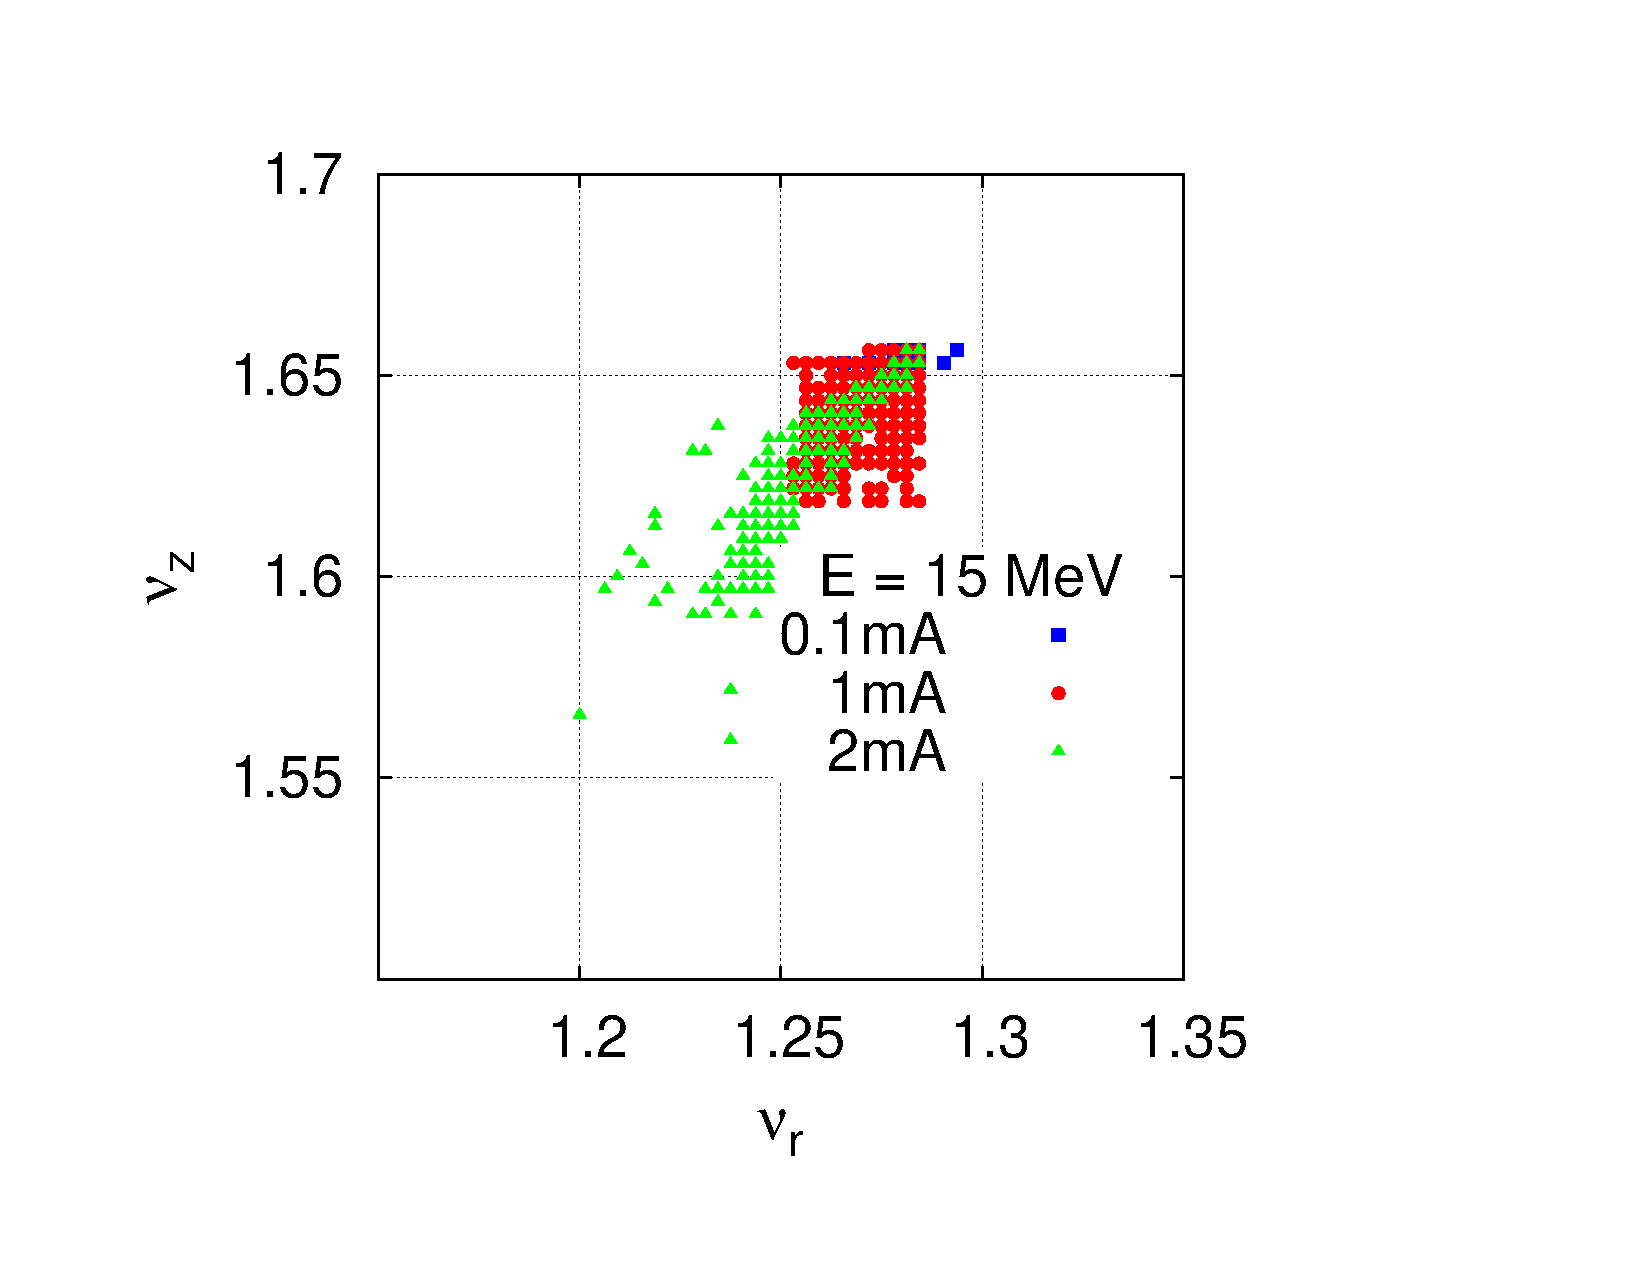
\includegraphics[width=0.49\linewidth,trim=2.5cm 2.5cm 6cm 0cm]{figures/nurnuz-15MeV.pdf}
%    \includegraphics[width=0.49\linewidth,trim=2.5cm 2.5cm 6cm 2.5cm]{figures/nurnuz-35MeV.pdf}
%    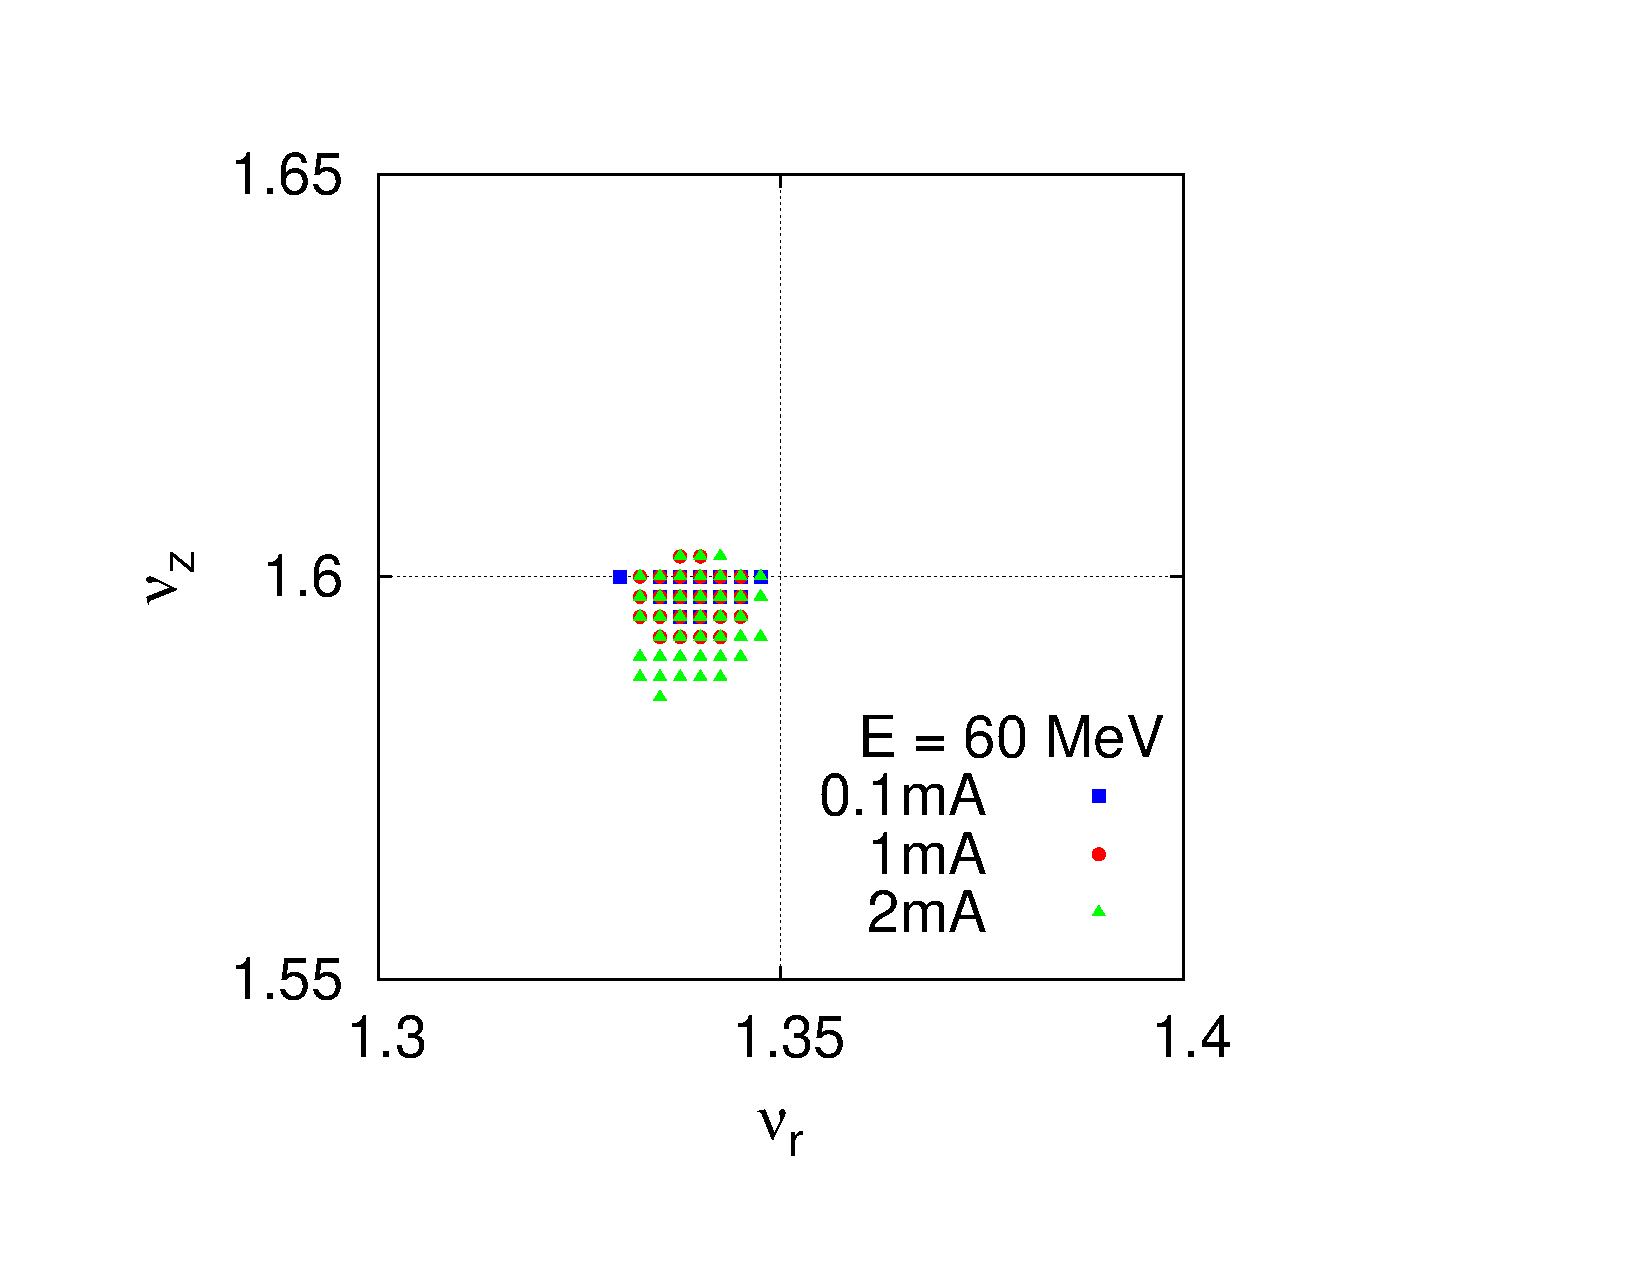
\includegraphics[width=0.49\linewidth,trim=2.5cm 2.5cm 6cm 2.5cm]{figures/nurnuz-60MeV.pdf}
%    \caption{(Color) Transverse tune spread of 5, 10, 35 and 60\,MeV Energy beam in Injector\,II calculated by \opalcycl. 
%      The square symbols correspond to a average current of 0.1 mA, the red circle symbols to 1 mA and the green triangle symbols to 2 mA.}
%    \label{fig:tuneSC}
%\end{figure*}


\section{APPLICATIONS}

\subsection{Different phase width studies of the PSI Ring Cyclotron}

Although a very compact beam with a phase width of about $2^\circ$ can be extracted from the Injector\,II, it is nevertheless subject to expansion in the longitudinal direction in the 72\,MeV 
beam transfer line because of space charge effects and chromatic dispersion. For the future 3\,mA beam, this will have a significant impact on the beam dynamic of the Ring cyclotron.
In response, a rebuncher running on the 10$th$ harmonic is planed to be installed on the beam line to make bunches as short as possible at the injection point of the Ring.
The final bunch length achieved is a critical aspect of the Ring cyclotron.
%Therefore, how short the bunch should be achieved at the injection point of the Ring is a critical question. 

In order to obtain a clear perspective on this issue, \opalcycl \  was applied to do numerical simulation on the Ring  by tracking Gaussian type beams with 3
different initial conditions. The initial longitudinal phase widths (6$\sigma$) are set to $2^\circ$, $6^\circ$ and $10^\circ$, respectively,
and the initial energy spread is neglected.
The initial conditions on the horizontal and vertical directions are the same. 
%On the horizontal direction, the beam sizes are $12$\,mm and momenta are set to zero. On the vertical direction, beam sizes and momenta are $12$\,mm and $3.4\times10^{-4}$. 
The initial distribution is not correlated in phase space.
The simulation used $10^6$ macro-particles and 32$\times$32$\times$32 gird sizes. The peak voltage of the main resonator and the 3rd harmonic flat-top resonator are 0.9\,MV and
0.403\,MV (11.2\% of accelerating voltage), respectively. The time step is set to 0.1 ns. It takes about 7 hours on CRAY XT3 of CSCS using 64 processors to track particles from the 
injection to the extraction.

\begin{figure*}
  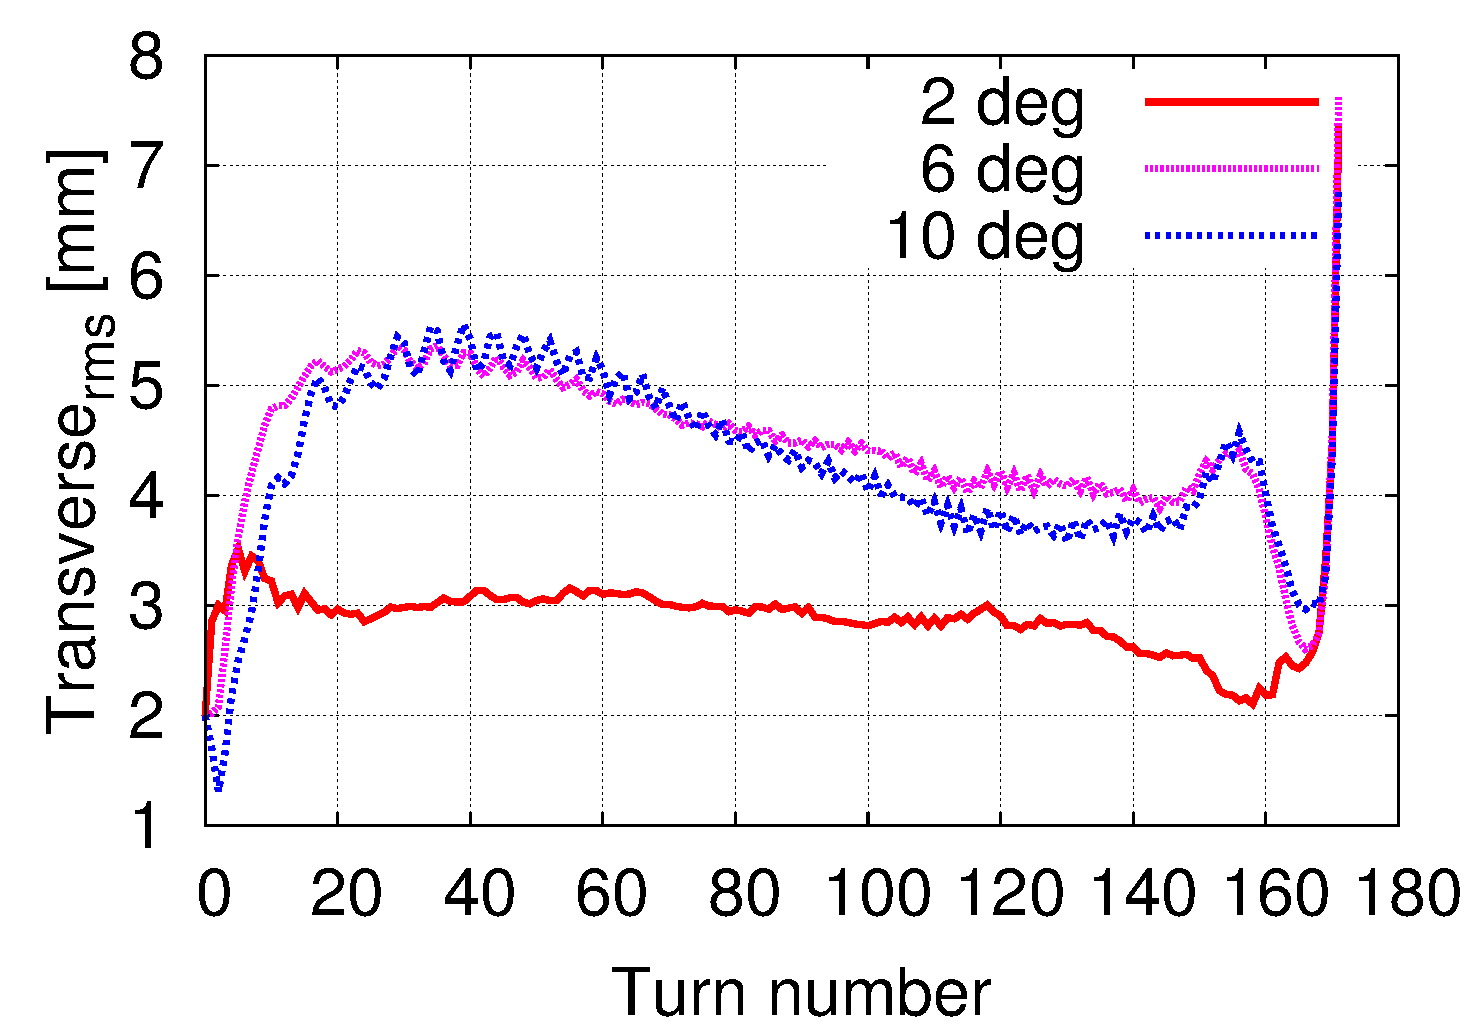
\includegraphics[width=0.45\linewidth]{figures/Comp-Transverse.pdf}
  \includegraphics[width=0.45\linewidth]{figures/Comp-Longitudinal.pdf}
  \caption{(Color) Comparison of the rms beam size in the transverse direction (left) and longitudinal direction (right) at $112^\circ$ azimuthal position of each turn 
    in PSI Ring cyclotron. }
  \label{fig:RMSsize}
\end{figure*}

\begin{figure*}
  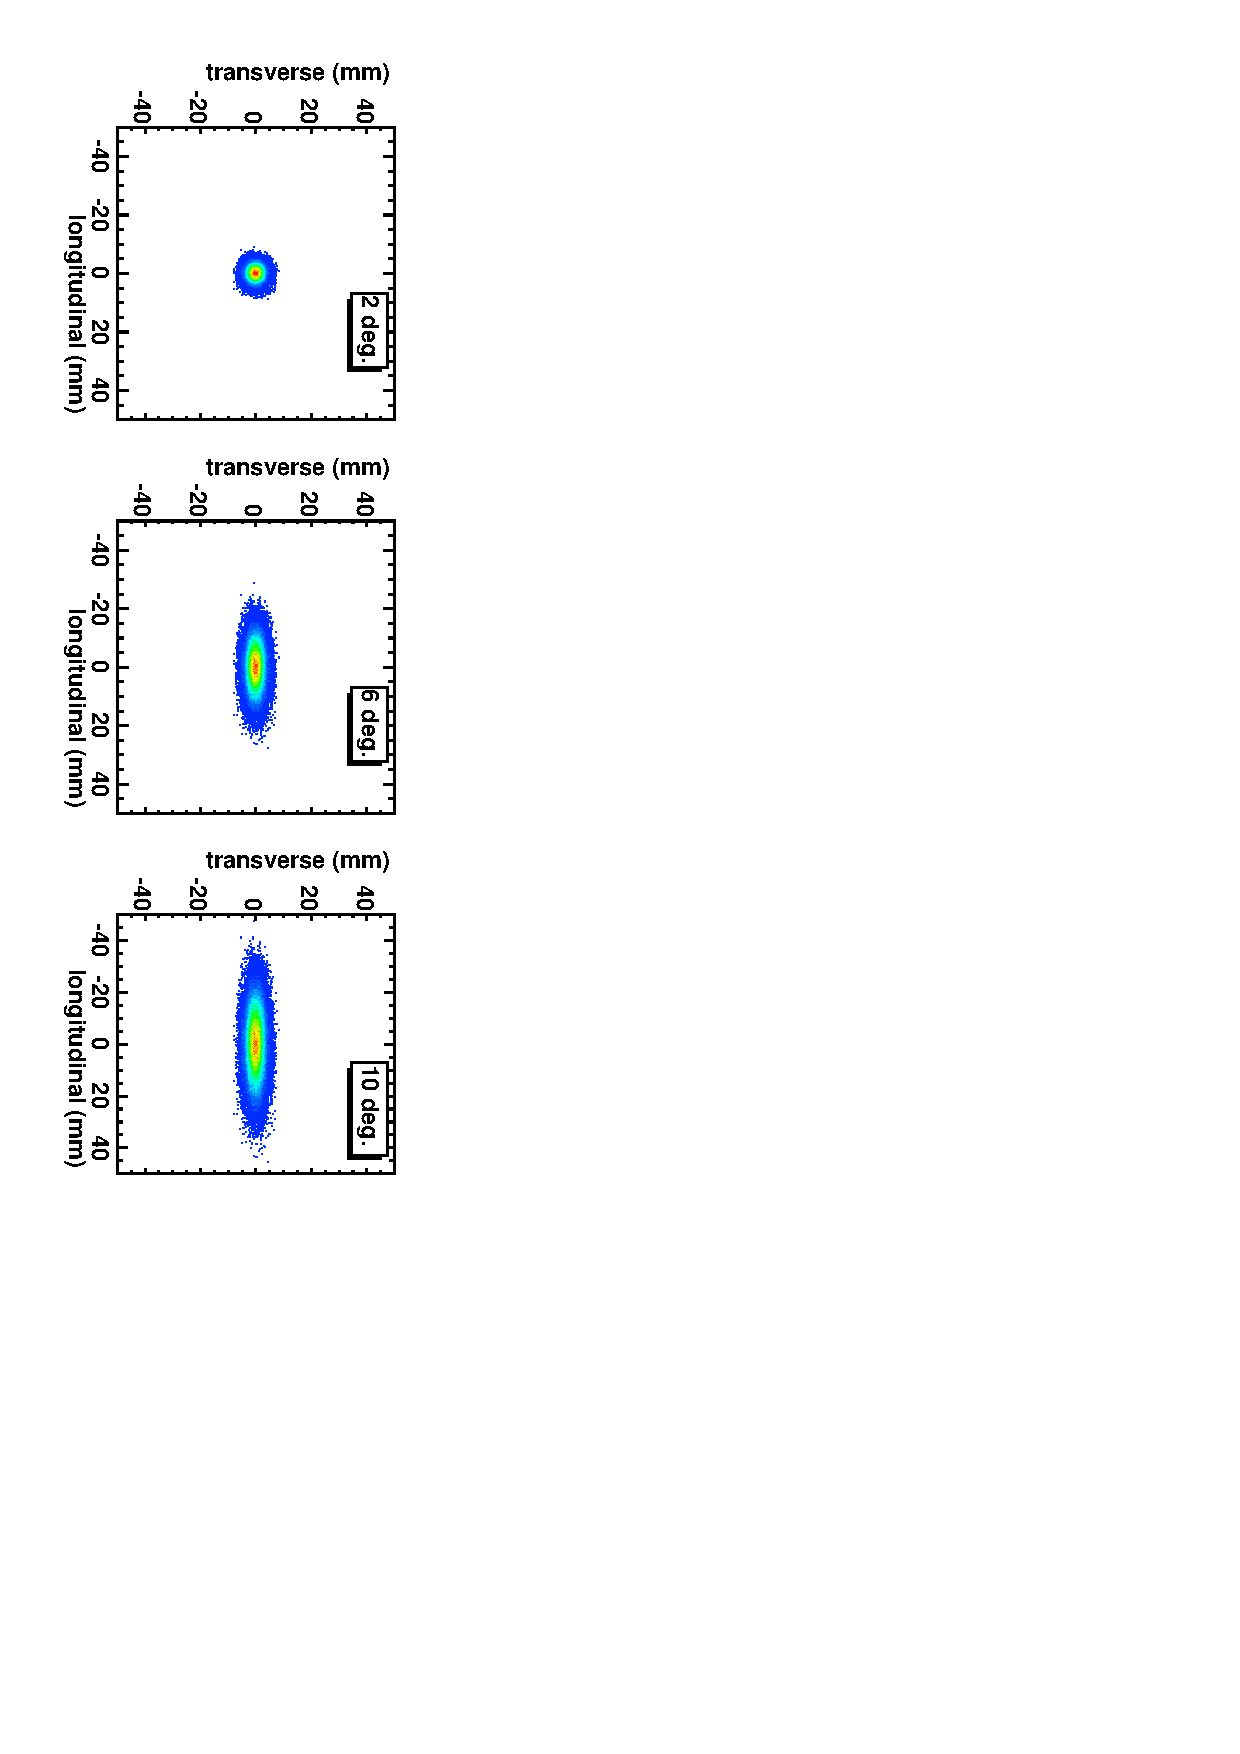
\includegraphics[angle=90,width=0.9\linewidth]{figures/Turn-0.pdf}
  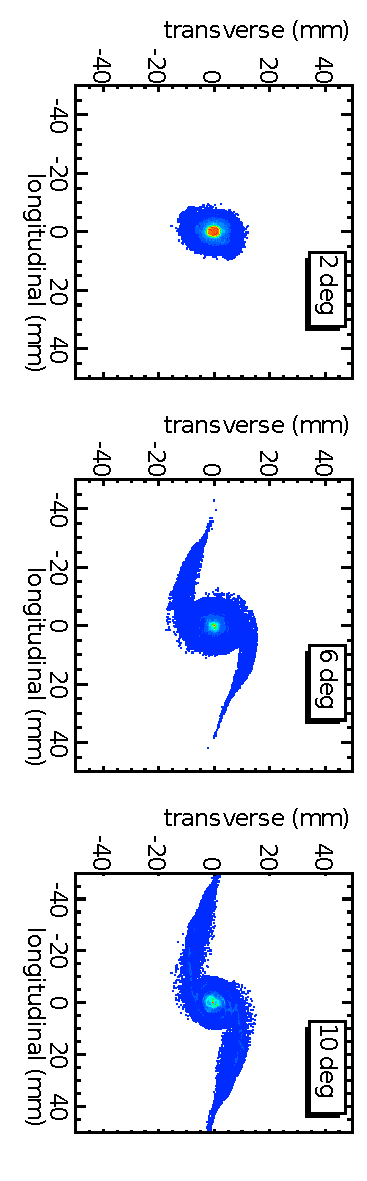
\includegraphics[angle=90,width=0.9\linewidth]{figures/Turn-50.pdf}
  \includegraphics[angle=90,width=0.9\linewidth]{figures/Turn-150.pdf}
  \caption{(Color) Top view of 3\,mA bunch distributions with  $2^\circ$, $6^\circ$ and $10^\circ$ initial phase widths at the initial position(top) turn 50 (middle), and 150 (bottom) 
    in the local frame ${\bs{S}_{local}}$ of $112^\circ$ azimuthal position of PSI Ring cyclotron. }
  \label{fig:RingPhaseWidth}
\end{figure*}

\begin{figure*}
  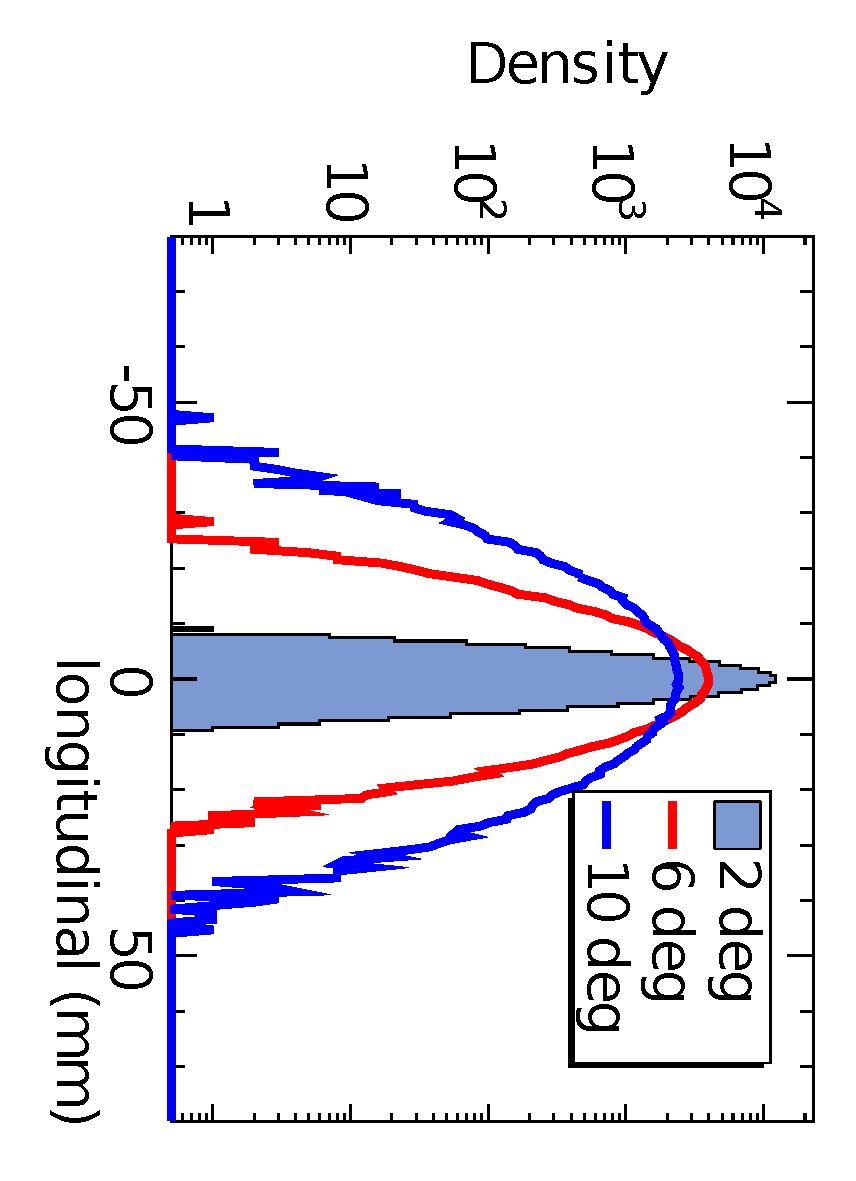
\includegraphics[angle=90,width=0.3\linewidth]{figures/Theta-Turn-0.pdf}
  \includegraphics[angle=90,width=0.3\linewidth]{figures/Theta-Turn-50.pdf}
  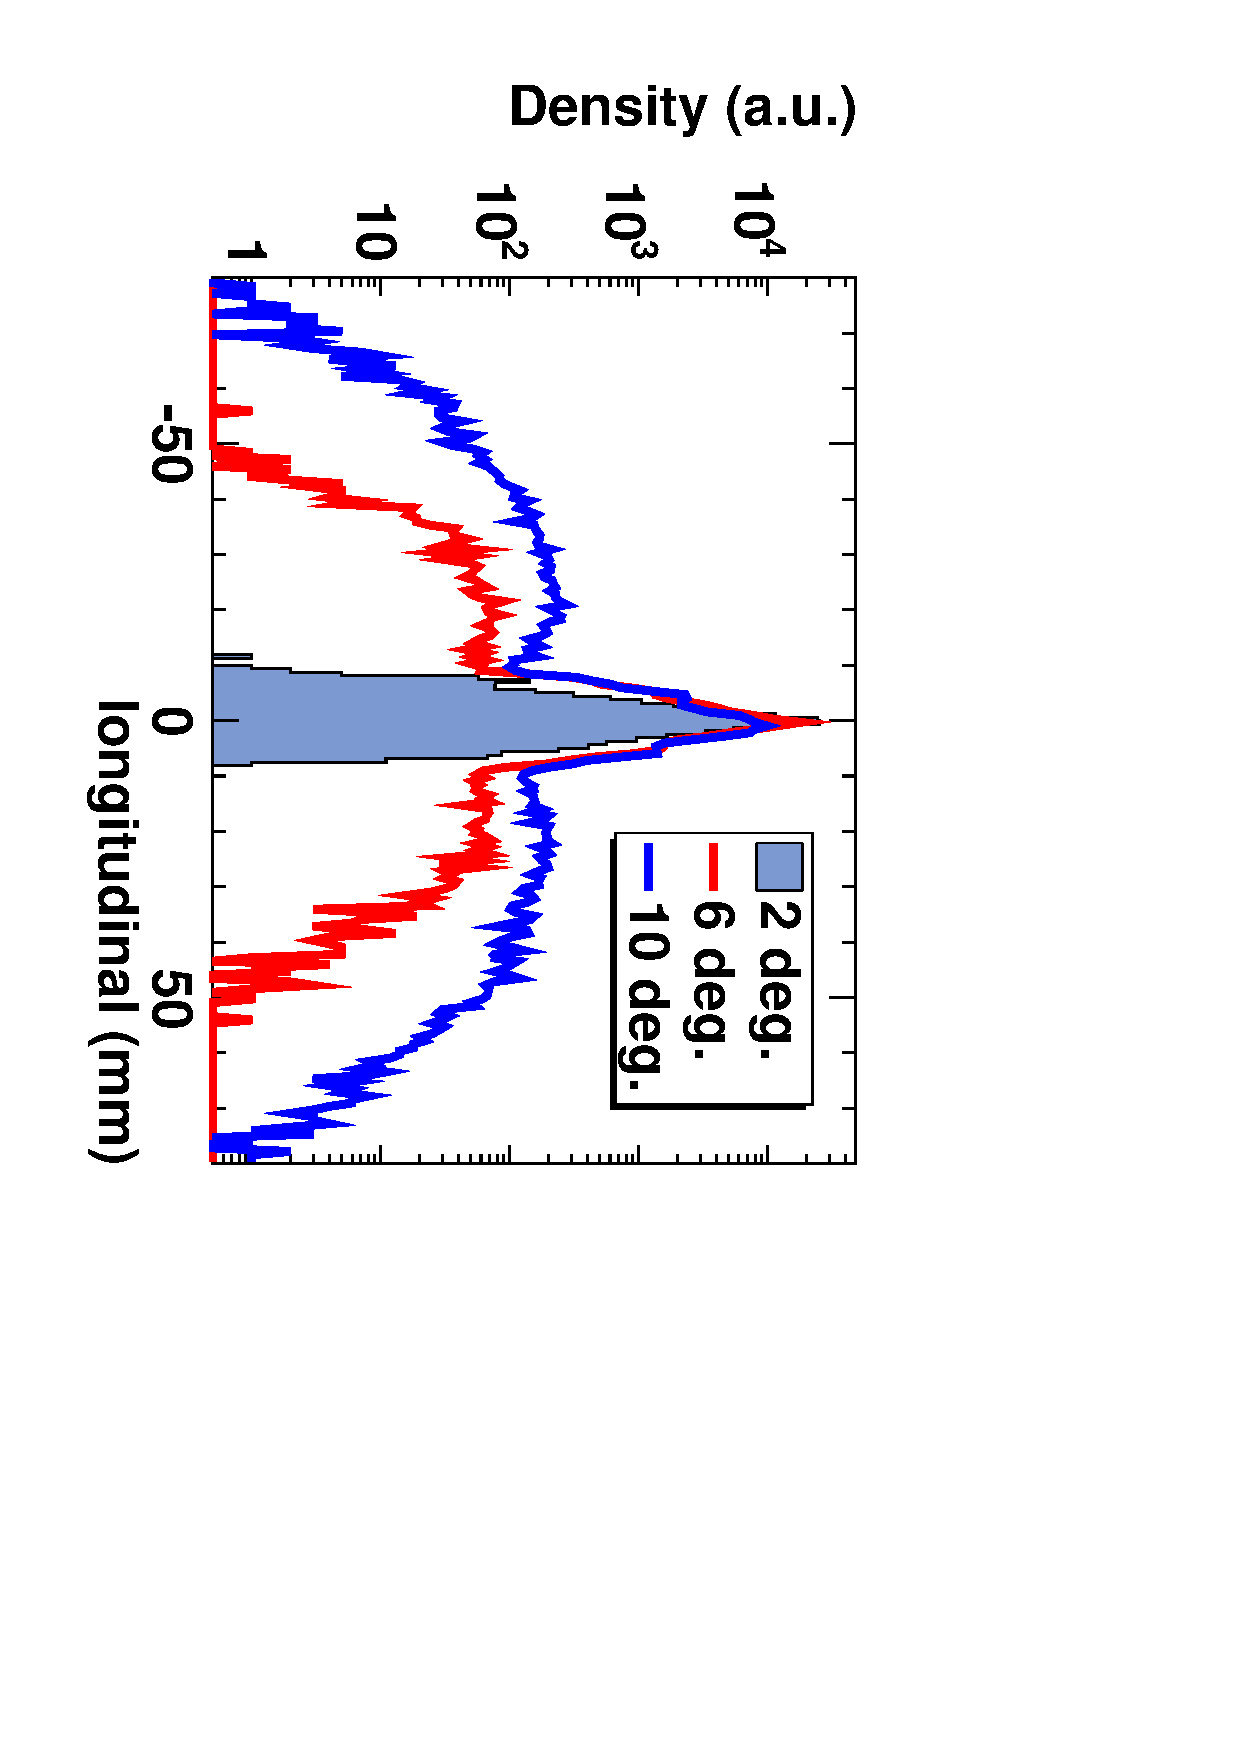
\includegraphics[angle=90,width=0.3\linewidth]{figures/Theta-Turn-150.pdf}
  \caption{(Color) Histogram of 3\,mA bunch distributions with  $2^\circ$, $6^\circ$ and $10^\circ$ initial phase widths at initial position(left), turn 50 (middle), and 150 (right) in PSI Ring cyclotron.}
  \label{fig:ThetaHitgram}
\end{figure*}

Fig.\,\ref{fig:RMSsize} shows the development of the beam rms size on the transverse and the longitudinal direction. We can see the beam is compressed
gradually in the longitudinal direction. Meanwhile in the transverse direction, the beam size increases fast during the first several turns 
because of the mismatch of initial conditions. Thereafter the beam size  does not change significantly until the beam arrives at the extraction region 
where it is distorted by the external magnetic field (extraction bump).
Fig.\,\ref{fig:RingPhaseWidth} shows the projection of phase space onto the middle plane of machine, and 
Fig.\,\ref{fig:ThetaHitgram} plots the histogram along the longitudinal direction at $112^\circ$ azimuthal position of turn 0, 50 and 150.
We can see for the bunch with the initial phase width of $2^\circ$, the bunch maintains a very compact shape with a stable round core without haloes. 
When the initial phase width increases, the size of the core only widens slightly (less than 5\,mm), while the spiral tails expand in the longitudinal direction and 
are unable to develop stable haloes. However, the beam does not expands notably in the radial direction, which means no substantial increase of the beam loss 
on the extraction septum is expected for the bunch with initial phase width less than $10^\circ$.

\subsection {Neighboring bunch effects in the PSI Ring}

As discussed in section I, neighboring bunch effects may have an appreciable influence on beam dynamics in the Ring. This can be evaluated by comparing the difference in single bunch and multiple bunch simulations as 
described in section III. We tested for 3, 5, 7 and 9 bunches and found that 
the difference between the 7 bunch scenario and that of 9 bunch scenarios is small, i.e. is viewed as converged,  as illustrated in Fig.\,\ref{fig:NBcompare2D}. 
As is evident from Fig.\,\ref{fig:NBcompare}, the FWHM of the beam transverse profile from the multi-bunch simulation is 1\,mm narrower than that of a single bunch, and the FWHM of energy spread is also slightly reduced. 

This phenomenon can be physically explained as follows. For an individual particle in the objective bunch, the space charge force from the neighboring bunches at the smaller radius is outward;
while the space charge force from the neighboring bunches at the larger radius is inward. For the particle in the center of the objective bunch, 
the forces in both directions are almost the same, hence there is no obvious influence brought to the particle. For the particles with a radius smaller than the center particle, 
the outward force is stronger than the inward force, so they will move outwards; for the particles with an radius larger than the center particle, 
the inward force is stronger than the outward force, so they will move inwards. Therefore,
more particles are distributed close to the bunch center and the bunch size is reduced in the radial direction.
%a squeezing force is exerted on it in the radial direction and as a consequence,  looking at the whole bunch, 


From the comparison, we conclude that neighboring bunch effects impose visible impacts on the beam dynamics for beam currents beyond 1\,mA in the PSI Ring. 
The bunch becomes more compact in the transverse direction and the energy spread is slightly reduced. Therefore neighboring bunch effects have a positive influence
on reducing beam loss in high intensity operation.

\begin{figure*}
  \includegraphics[width=1\linewidth]{figures/C9B7BSB-2D-1mA-130.pdf}
  \caption{(Color) Top view of 1\,mA bunch distributions at the turn 130  in the local frame ${\bs{S}_{local}}$ at $112^\circ$ azimuthal position of turn 130 in PSI Ring cyclotron.
    The results are obtained from single bunch (left), 7 bunches (middle) and 9 bunches (right) simulations, respectively.}
  \label{fig:NBcompare2D}
\end{figure*}

\begin{figure*}
  \includegraphics[angle=90,width=0.45\linewidth]{figures/C9B7BSB-R-1mA-130.pdf}
  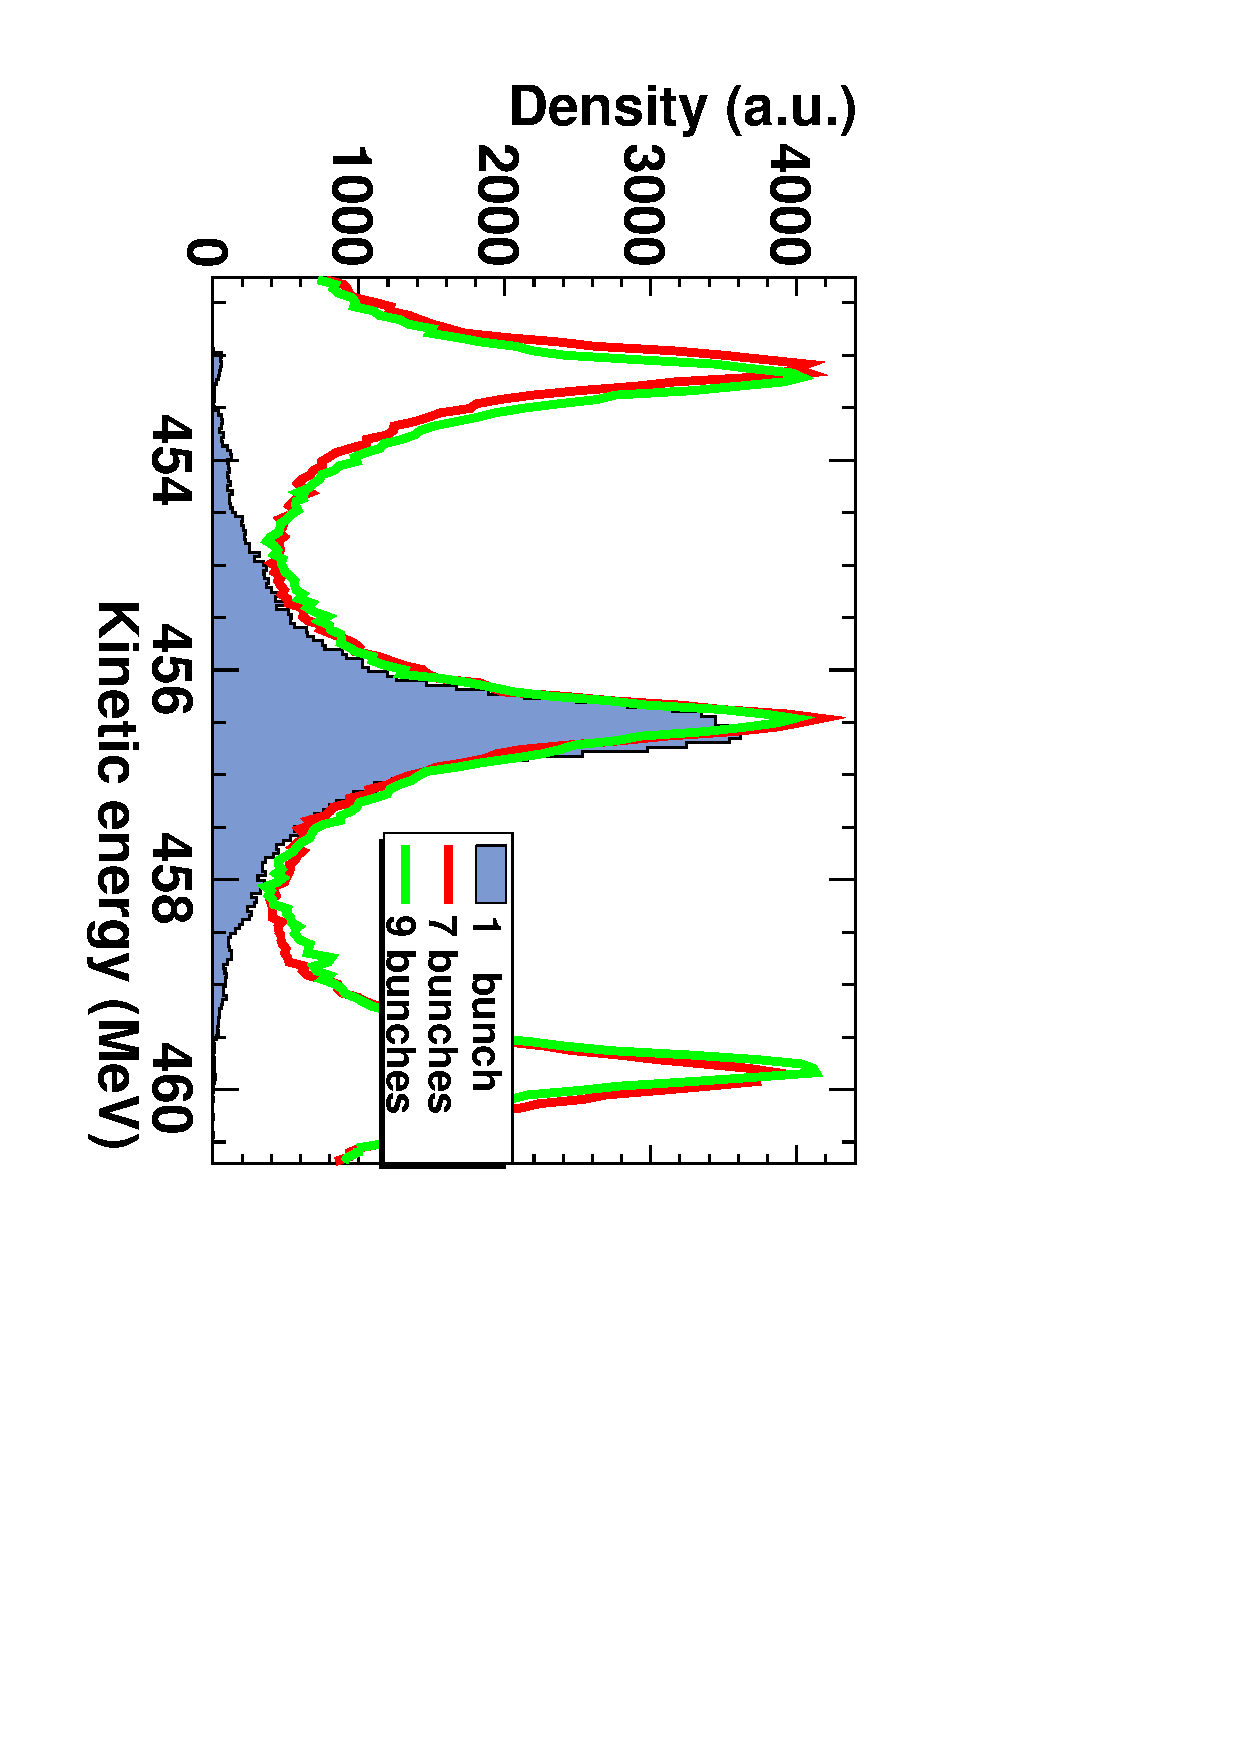
\includegraphics[angle=90,width=0.45\linewidth]{figures/C9B7BSB-Energy-1mA-130.pdf}
  \caption{(Color) Comparison of the histograms along the transversal direction in the local frame ${\bs{S}_{local}}$ (left) and the energy spectra (right) of 1\,mA beam
    at $112^\circ$ azimuthal position of turn 130 in PSI Ring cyclotron.}
  \label{fig:NBcompare}
\end{figure*}

\section{CONCLUSIONS AND DISCUSSIONS}
In this paper, we presented a model for the beam dynamics in high intensity cyclotrons, which includes for the first time the space charge effects
of neighboring bunches in a self-consistent way. This model is implemented in an object-oriented three-dimensional parallel PIC code, 
as a flavor of the \opal\, framework. 

The performance tests on the CRAY XT3, CSCS demonstrate a good scalability of this code with respect to the number of used processors. 
The three operation modes of this code (tune calculation, single and multi particle mode) were validated by code comparison. This code has been successfully applied to study the behavior of the PSI Ring cyclotron at high intensities.

The beam intensity of this high power facility is practically limited by uncontrolled losses at the extraction element of the cyclotron, originating from beam tails that are developed during the acceleration process.
As the results show, the generation of beam tails can be avoided if short bunches with a phase length of $2^\circ$  or less are injected. 
An upgrade plan is under way to generate such short bunches with the help of a 10$th$ harmonic buncher.
Furthermore it is observed that the neighboring bunch effects can help to narrow the transverse beam size and reduce the energy spread.

It is planned to refine these simulations within the next year by a more detailed determination of the initial particle distribution at the injection
of the PSI Ring cyclotron. A quantitative comparison of the results with measured beam properties will be presented in a future paper.
%Perform the first parallel simulation of multiple bunches in cyclotron
%Study neighboring bunch effects on the beam's evolution quantitatively on PSI Ring cyclotron
\section{ACKNOWLEDGMENTS}
The authors thank the Accelerator Modeling and Advanced Computing group members C.\,Kraus, Y.\,Ineichen and B.\,Oswald for many 
discussions regarding programming and T.\,Schietinger for providing the post-processing tool
H5PartRoot. We also thank W.\,Joho, S.\,Adam and R.\,D\"olling for many useful discussions regarding high
intensity beam dynamics in cyclotrons. This work was performed on the Merlin3 cluster at the Paul Scherrer Institut 
and on the Cray XT3 at Swiss National Supercomputing Center (CSCS) within the ``Horizon'' collaboration. One author (J.\,J.\,Yang) 
was partially supported by Natural Science Foundation of China (10775185) during his sabbatical at PSI.

% If in two-column mode, this environment will change to single-column
% format so that long equations can be displayed. Use
% sparingly.
%\begin{widetext}
% put long equation here
%\end{widetext}

% figures should be put into the text as floats.
% Use the graphics or graphicx packages (distributed with LaTeX2e)
% and the \includegraphics macro defined in those packages.
% See the LaTeX Graphics Companion by Michel Goosens, Sebastian Rahtz,
% and Frank Mittelbach for instance.
%
% Here is an example of the general form of a figure:
% Fill in the caption in the braces of the \caption{} command. Put the label
% that you will use with \ref{} command in the braces of the \label{} command.
% Use the figure* environment if the figure should span across the
% entire page. There is no need to do explicit centering.

% \begin{figure}
% \includegraphics{}%
% \caption{\label{}}
% \end{figure}

% Surround figure environment with turnpage environment for landscape
% figure
% \begin{turnpage}
% \begin{figure}
% \includegraphics{}%
% \caption{\label{}}
% \end{figure}
% \end{turnpage}

% tables should appear as floats within the text
%
% Here is an example of the general form of a table:
% Fill in the caption in the braces of the \caption{} command. Put the label
% that you will use with \ref{} command in the braces of the \label{} command.
% Insert the column specifiers (l, r, c, d, etc.) in the empty braces of the
% \begin{tabular}{} command.
% The ruledtabular enviroment adds doubled rules to table and sets a
% reasonable default table settings.
% Use the table* environment to get a full-width table in two-column
% Add \usepackage{longtable} and the longtable (or longtable*}
% environment for nicely formatted long tables. Or use the the [H]
% placement option to break a long table (with less control than 
% in longtable).
% \begin{table}%[H] add [H] placement to break table across pages
% \caption{\label{}}
% \begin{ruledtabular}
% \begin{tabular}{}
% Lines of table here ending with \\
% \end{tabular}
% \end{ruledtabular}
% \end{table}

% Surround table environment with turnpage environment for landscape
% table
% \begin{turnpage}
% \begin{table}
% \caption{\label{}}
% \begin{ruledtabular}
% \begin{tabular}{}
% \end{tabular}
% \end{ruledtabular}
% \end{table}
% \end{turnpage}

% Specify following sections are appendices. Use \appendix* if there
% only one appendix.
%\appendix
%\section{}

% If you have acknowledgments, this puts in the proper section head.
%\begin{acknowledgments}
% put your acknowledgments here.
%\end{acknowledgments}

% Create the reference section using BibTeX:
\bibliography{Refbase}

\end{document}
%
% ****** End of file template.aps ******

